\section{Story Patterns} 
\label{sec:StoryPatterns}

In this section, we introduce story patterns in more detail.
We start by giving the general idea of story patterns in Section \ref{sec:StoryPatterns:storyPattern}.
Thereafter, we describe the basic concepts of story patterns, namely object variables, link variables,
and their respective binding semantics in Sections \ref{sec:StoryPatterns:objects} to \ref{sec:StoryPatterns:binding}.
Finally, we show the use of object attributes in a story pattern in Section \ref{sec:StoryPatterns:attributes}.


\subsection{General Idea}
\label{sec:StoryPatterns:storyPattern}

Story patterns are typed attributed graph transformation rules with inheritance on object types (cf. Section~\ref{sec:foundations:typedAttrGTS}) that can be embedded into an activity node of a story diagram (cf. Section~\ref{sec:StoryDiagrams}).
 By using a type model as introduced in Section~\ref{sec:foundations:typedAttrGTS}, story patterns enable polymorphism for matching object and link variables.
This allows for specifying graph replacement rules for object-oriented models.

Object and link variables are matched to the objects and links of the instance model. 
In contrast to typed attributed graph transformations, story patterns explicitly require to use isomorphic matchings, i.e., two object variables of a story pattern may not be matched to the same object of the instance model.

For enabling a concise notation of the graph transformation, story patterns apply a short-hand notation depicting the left-hand side (LHS) and the right-hand side (RHS) in a single, annotated graph using stereotypes.
In the short-hand notation, we use binding operators for defining the LHS and the RHS. Object and link variables representing objects and links not to be changed by the story pattern carry no stereotype. 
Object and link variables representing objects to be created (or deleted) are annotated with \create (or  \destroy, respectively). 
Consequently, the LHS consists of all object and link variables that carry no stereotype or stereotype \destroy. The RHS consists of all object and link variables that carry no stereotype or the stereotype \create.
The deletion of objects and links follows the single-pushout approach (cf.\ Section~\ref{sec:foundations:simpleGTS}).

Figure \ref{fig:simpleStoryPattern} shows an example of a single story pattern that redirects a method call from an old method to a new method.
\begin{figure}[htb]
  \centering
  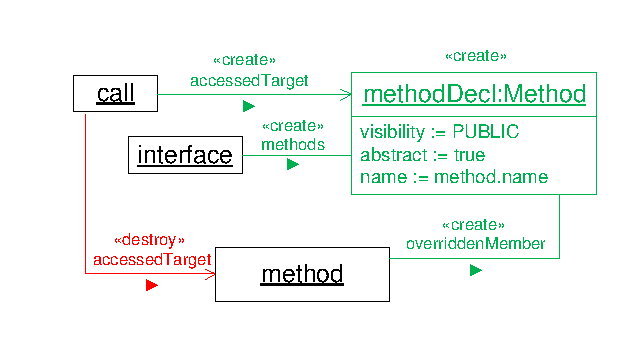
\includegraphics[scale=1.0]{figures/SimpleStoryPattern}
  \caption{Example of a Story Pattern}
  \label{fig:simpleStoryPattern}
\end{figure}
In the example, the object variables \fe{parentClass}, \fe{oldMethod}, and \fe{newMethod} are bound variables, i.e., they already refer to objects of the instance model (cf. Section \ref{sec:StoryPatterns:binding:states}).
The object variables \fe{anyMethod} and \fe{c} are unbound. 
When applying the story pattern, first a match for \fe{anyMethod} and \fe{c} is searched in the instance graph. 
A possible match will be any method in \fe{parentClass} which contains a call to \fe{oldMethod}. 
If the matching is successful, the link from \fe{c} to \fe{oldMethod} will be deleted and the link from \fe{c} to \fe{newMethod} will be created.

In the concrete syntax of story patterns, the object and link variables representing objects and links not to be modified by the story pattern are visualized in black. 
Object and link variables representing objects and links to be destroyed are annotated with \destroy and visualized in red. 
Object and link variables representing objects and links to be created are annotated with \create and visualized in green. 
An unbound object variable is labeled with its name and the name of the corresponding type. 
For bound object variables, we omit the name of the type (e.g.\ \fe{parentClass} in Figure~\ref{fig:simpleStoryPattern}).

In general, the matching process is executed as a three step process:
first, a matching is searched which uses the bound variables of the story pattern as a starting point. The matching associates objects and links of the instance model to all object and link variables of the story pattern. 
The matching is performed as defined for typed attributed graph transformations and considers all object and link variables of the LHS.
If a matching can be obtained, the story pattern is applicable and the execution proceeds. 
\tododt{What happens if the modification operations are contradictory (see Section~\ref{sec:DecisionNodesEtc})?}
Otherwise the execution of the story pattern is aborted.
In the second step, all objects and links matched to object and link variables annotated with \destroy are deleted. 
Finally, objects and links are created in the instance model for all variables annotated with \create.

Story patterns aim to reduce the computational complexity of the matching process (cf. Section~\ref{sec:foundations:simpleGTS}) by using bound variables.
We require at least one bound object variable in each story pattern which is used as a starting point for the matching process.


\subsection{Objects and Object Variables}
\label{sec:StoryPatterns:objects}

Object variables in a story pattern represent the objects in an instance model to be matched.
The variables are uniquely identified by their name.
The objects are instances of classes of the underlying type model (cf.
Section \ref{sec:foundations:typedAttrGTS}). Thus, the object variables are typed by classes from this model.

The story pattern in Figure \ref{fig:simpleStoryPattern} contains five
object variables with the names \fe{parentClass}, \fe{oldMethod}, \fe{anyMethod}, \fe{c} and
\fe{newMethod}. 
The type of an object variable is only visualized if the
variable is unbound or maybe bound (cf.\ Section
\ref{sec:StoryPatterns:binding:states}). For example, the object variable \fe{anyMethod} has the type \fe{Method}.

Object variables have binding states, binding operators and binding semantics which are described in Section  \ref{sec:StoryPatterns:binding}.


\ext %--- Comment this line to include primitive variables into the document
{
\todomcp{Primitive Variables: concrete syntax like
object variables; binding expressions for initialization, see figure
\ref{fig:primitiveVariable}; primitive variables are typed over EDataType; they
exist to the end of the Activity}

\begin{figure}[htb]
  \centering
  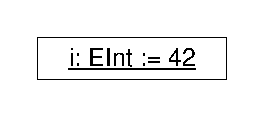
\includegraphics[scale=0.6]{figures/PrimitiveVariable}
  \caption{Primitive variable with value assignment}
  \label{fig:primitiveVariable}
\end{figure}

\todomcp{Links to primitive variables: special LinkVariable, typed over
EStructuralFeature}
}%------ End of primitive variables section



\subsection{Links and Link Variables}
\label{sec:StoryPatterns:links}

Link variables represent connections between objects and are used to connect
different object variables. A link variable is typed over a reference of the underlying
type graph.

Like object variables, link variables also have binding
operators and binding semantics (cf. Section \ref{sec:StoryPatterns:binding}), but no binding state.




\subsection{Binding of Variables}
\label{sec:StoryPatterns:binding}

Object variables have binding states (unbound, bound, maybe
bound), binding semantics (mandatory, negative, optional), and binding operators
(check only, create, destroy). Link variables have binding
operators and binding semantics.
Their meaning is described in the following. 


\subsubsection{Binding States}
\label{sec:StoryPatterns:binding:states}

An object variable or a link variable can be declared as \emph{bound}, \emph{unbound}, or
\emph{maybe bound} (i.e. it is unknown if the variable is bound or not). This is
defined by its binding state. An unbound variable is matched during the
execution of the containing story pattern. 
A bound variable must have been matched previously. 
For a variable that is specified as maybe bound, a new match will only be
determined if it has not been bound before. 
Otherwise it will be treated as a bound variable.
This is useful, if the same pattern should be used in different contexts, i.e., the bound variable of the pattern differs depending on the context but otherwise the patterns are identical.
Without maybe bound variables, different patterns would have to be modeled that only differ in which variable is the bound variable of the pattern.
With maybe bound variables, all variables can be set to maybe bound and the caller specifies a binding for one of them depending on the context.
%\todomcp{explain why maybe bound is necessary}

Unbound object variables are visualized with an underlined label of the form
``name: Type'' (cf. Figure \ref{fig:bindingStatesOverview} a)).
For bound object variables the type is hidden, as depicted
in Figure \ref{fig:bindingStatesOverview} b).
Maybe bound object variables are represented like unbound object variables, but
are marked by a question mark after the name (cf.\ Figure
\ref{fig:bindingStatesOverview} c)).

In a valid story pattern, each connected component\footnote{With
``connected component'' we mean a subgraph in which each object variable is
reachable from at least one bound object variable via directed link variables.}
must contain at least one bound object variable or created variables only. This
is necessary to avoid a search over the whole underlying instance model which requires a long runtime in most cases (cf. Section~\ref{sec:StoryPatterns:storyPattern}).

\begin{figure}[htb]
  \centering
  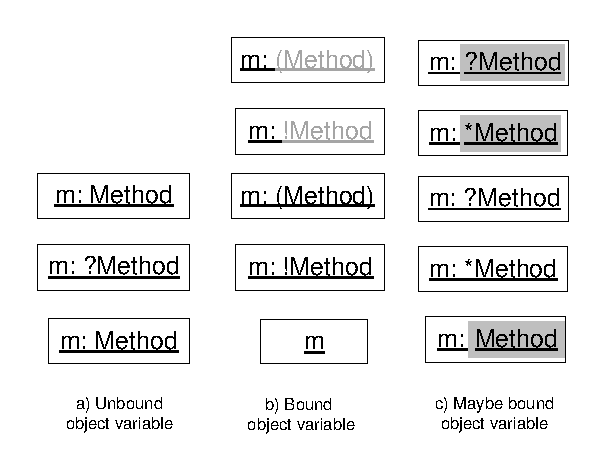
\includegraphics[scale=1.2]{figures/BindingStatesOverview}
  \caption{Binding States for Object Variables}
  \label{fig:bindingStatesOverview}
\end{figure}

\subsubsection{Binding Semantics}
\label{sec:StoryPatterns:binding:semantics}
Object variables and link variables have binding semantics that
determine if a variable is mandatory, negative or optional.
A match for mandatory variables must exist in the given instance model, otherwise
the pattern matching fails. 
In contrast, negative variables constitute so-called negative application
conditions (NACs) and must not exist in the instance model. If a variable defined as
negative can be matched during the execution of the story pattern, the pattern matching
fails. Matches for optional variables may exist. An optional variable will be
bound if possible, but the story pattern may also be matched
successfully otherwise.

Negative object variables are visualized crossed-out (cf. Figure
\ref{fig:bindingSemanticsOverview} b)) and optional object variables are
visualized with a dashed border (cf.\ Figure \ref{fig:bindingSemanticsOverview} c)).
The same holds for negative and optional link variables (cf. Figure
\ref{fig:bindingSemanticsOverview} e) and f)).

Negative as well as optional object and link variables are not part of a
connected component.
This means, the graph has to be still connected when ignoring optional and negative
parts. However, optional and negative object variables must be reachable from a connected component. 
Consequently, regarding the rule that each connected component must
contain at least one bound object variable (cf.\ Section
\ref{sec:StoryPatterns:binding:states}), there are situations in which the
use of negative or optional object variables is not allowed. 
Figure \ref{fig:negativeObjects} shows these situations. 
Case a) is allowed but case b) is not because, in the latter case,
the graph without the negative and optional elements is not a connected component anymore.
Case c) is allowed because the object
variables \fe{a} and \fe{c} are bound which means that each connected component has at least one bound object variable.
Accordingly, case d) is allowed, too, because \fe{a} and \fe{b} are both
bound. Case e) is not allowed while Case f) is.
Case g) is not allowed because the semantics is the same as in Case a) due to the single-pushout approach of story patterns.

Similar to the application of negative object
variables, Figure \ref{fig:optionalObjects} shows some examples for the application of optional object variables. 
While case a) is allowed, case b) is not allowed because in this case the
shown graph is not connected anymore. However, case c) and d) are allowed
because each connected component contains at least one bound object variable.
Cases e) and f) are also allowed.

\begin{figure}[htb]
  \centering
  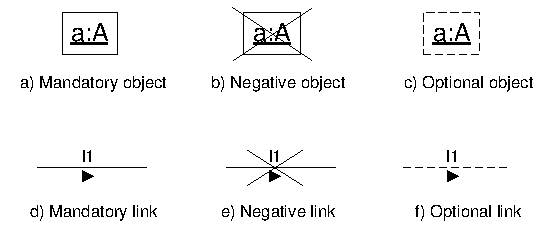
\includegraphics[scale=1.2]{figures/BindingSemanticsOverview}
  \caption{Binding Semantics for Object and Link Variables}
  \label{fig:bindingSemanticsOverview}
\end{figure}

\begin{figure}[htb]
  \centering
  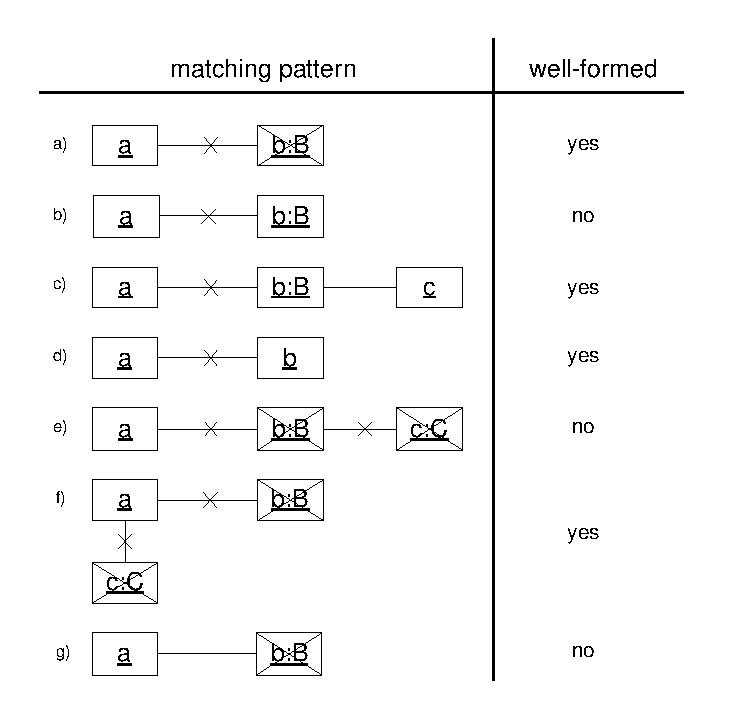
\includegraphics[scale=1]{figures/negativeObjects}
  \caption{Negative Application Conditions}
  \label{fig:negativeObjects}
\end{figure}

\begin{figure}[htb]
  \centering
  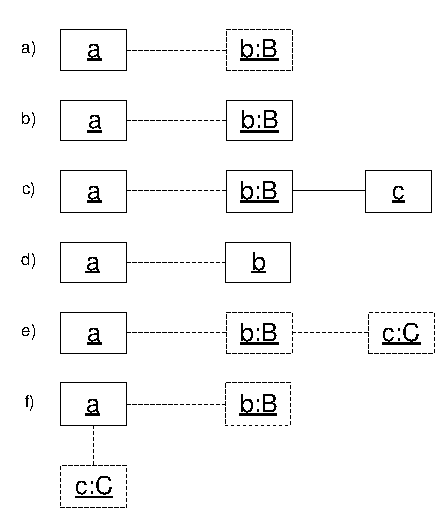
\includegraphics[scale=1]{figures/optionalObjects}
  \caption{Optional Object and Link Variables}
  \label{fig:optionalObjects}
\end{figure}


\subsubsection{Binding Operators}
\label{sec:StoryPatterns:binding:operators}

Binding operators define whether an object or link is to be created, deleted,
or just matched in the instance model.
After all elements that are defined to be deleted or just matched have been
matched, the model is modified by deleting and creating the elements as
defined (see Section~\ref{sec:StoryPatterns:storyPattern}).

Objects and links to be created are marked with the
stereotype \create (cf.\ Figure \ref{fig:bindingOperatorsOverview} b) and e)) and objects and links
to be deleted are marked with the stereotype \destroy (cf.\ Figure
\ref{fig:bindingOperatorsOverview} c) and f)).

\begin{figure}[htb]
  \centering
  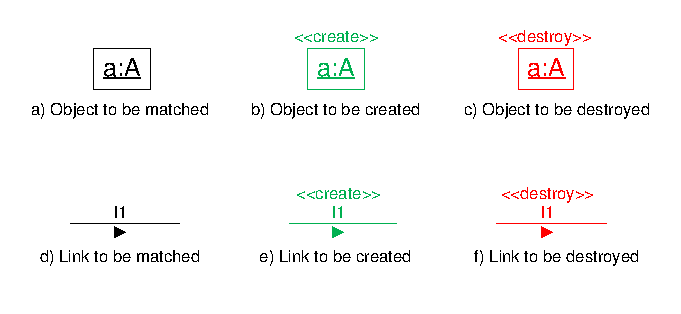
\includegraphics[scale=1.2]{figures/BindingOperatorsOverview}
  \caption{Binding Operators for Object and Link Variables}
  \label{fig:bindingOperatorsOverview}
\end{figure}

Since no objects and links exist for variables marked with \create, they also do not belong to a connected component (like
negative or optional variables).


\subsubsection{Feasible Binding Combinations}

Binding states, binding semantics and binding operators can be
arbitrarily combined, but only certain combinations are feasible. 
Table \ref{tab:bindingCombinations} lists all feasible binding combinations for
object variables. As shown there, bound and maybe bound object variables must not have negative
or optional binding semantics. As well, the combination of the binding states
bound or maybe bound and the binding operator create is not allowed.

% Table generated by Excel2LaTeX from sheet 'Tabelle1'
\begin{table}[htbp]
  \centering
  \caption{Feasible Combinations of Binding States, Binding Semantics, and
  Binding Operators for Object Variables}
    \begin{tabular}{|r|r|r|r|}
    \hline
    \textbf{Binding State} & \textbf{Binding Semantics} & \textbf{Binding
    Operator} & \textbf{Feasible} \\
    \hline
    UNBOUND & MANDATORY & CHECK\_ONLY & yes \\
    UNBOUND & MANDATORY & CREATE & yes \\
    UNBOUND & MANDATORY & DESTROY & yes \\
    UNBOUND & NEGATIVE & CHECK\_ONLY & yes \\
    UNBOUND & NEGATIVE & CREATE & no \\
    UNBOUND & NEGATIVE & DESTROY & no \\
    UNBOUND & OPTIONAL & CHECK\_ONLY & yes \\
    UNBOUND & OPTIONAL & CREATE & yes \\
    UNBOUND & OPTIONAL & DESTROY & yes \\
    \hline
    BOUND & MANDATORY & CHECK\_ONLY & yes \\
    BOUND & MANDATORY & CREATE & no \\
    BOUND & MANDATORY & DESTROY & yes \\
    BOUND & NEGATIVE & CHECK\_ONLY & no \\
    BOUND & NEGATIVE & CREATE & no \\
    BOUND & NEGATIVE & DESTROY & no \\
    BOUND & OPTIONAL & CHECK\_ONLY & no \\
    BOUND & OPTIONAL & CREATE & no \\
    BOUND & OPTIONAL & DESTROY & no \\
    \hline
    MAYBE\_BOUND & MANDATORY & CHECK\_ONLY & yes \\
    MAYBE\_BOUND & MANDATORY & CREATE & no \\
    MAYBE\_BOUND & MANDATORY & DESTROY & yes \\
    MAYBE\_BOUND & NEGATIVE & CHECK\_ONLY & no \\
    MAYBE\_BOUND & NEGATIVE & CREATE & no \\
    MAYBE\_BOUND & NEGATIVE & DESTROY & no \\
    MAYBE\_BOUND & OPTIONAL & CHECK\_ONLY & no \\
    MAYBE\_BOUND & OPTIONAL & CREATE & no \\
    MAYBE\_BOUND & OPTIONAL & DESTROY & no \\
    \hline
    \end{tabular}%
  \label{tab:bindingCombinations}%
\end{table}%

%\todomcp{see albert's habil for example for optional-create}

%\todomcp{table for object set variables?}

\begin{table}[htbp]
  \centering
  \caption{Feasible Combinations of Binding Semantics and
  Binding Operators for Link Variables}
    \begin{tabular}{|r|r|r|}
    \hline
    \textbf{Binding Semantics} & \textbf{Binding
    Operator} & \textbf{Feasible} \\
    \hline
    MANDATORY & CHECK\_ONLY & yes \\
    MANDATORY & CREATE & yes \\
    MANDATORY & DESTROY & yes \\
    NEGATIVE & CHECK\_ONLY & yes \\
    NEGATIVE & CREATE & no \\
    NEGATIVE & DESTROY & no \\
    OPTIONAL & CHECK\_ONLY & yes \\
    OPTIONAL & CREATE & yes \\
    OPTIONAL & DESTROY & yes \\
    \hline
    \end{tabular}%
  \label{tab:bindingCombinations_links}%
\end{table}%

The feasible combinations of binding semantics and binding operators for link
variables are given in Table \ref{tab:bindingCombinations_links}. Link variables
have no binding state.


\subsection{Using Object Attributes}
\label{sec:StoryPatterns:attributes}

The objects of our instance model carry attributes. 
During the application of a story pattern, these attributes can be used twofold. 
First, attribute constraints can be specified to restrict the attribute values to a certain range, thereby restricting the possible matches of a story pattern. 
Second, attribute values can be changed during the graph rewriting step after a successful matching.

We use \emph{attribute constraints} to restrict the matching of object variables to objects of the instance model that have specific attribute values. 
Thus, attribute constraints are considered to be part of the LHS and do not change the instance model. 
The attribute constraints of an object variable are checked directly after matching the object variable. 
Figure \ref{fig:objectConstraint} shows an example.

\begin{figure}[htbp]
  \centering
  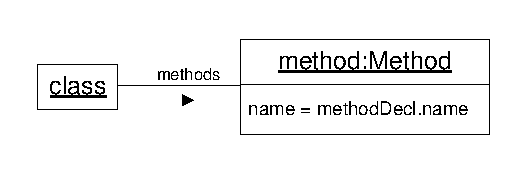
\includegraphics[scale=1]{figures/ObjectConstraint}
  \caption{Matching Pattern with an Attribute Constraint}
  \label{fig:objectConstraint}
\end{figure}

In the example, we match a method being contained in the class represented by the object variable \fe{theClass}. 
The match is restricted to a method which has the name "getName".

The values of attributes that are not restricted by an attribute constraint are not considered during the matching. 
Thus, they may have an arbitrary value. 
In the current version of story patterns, attribute constraints need to be specified using OCL~\cite{OCL}. 
Besides equality checks, all comparative operations on the attributes of an object supported by OCL can be used as object constraints. 

Besides attribute constraints, \emph{attribute assignments} can be used to change the value of an attribute during the application of a story pattern. 
Thus, attribute assignments are considered to be part of the RHS. 
When using attribute assignments, the value of the attribute is not considered while matching the LHS to the instance model. 
Figure \ref{fig:attributeAssignment} shows an example.

\begin{figure}[htbp]
  \centering
  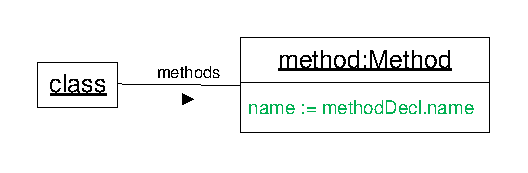
\includegraphics[scale=1]{figures/AttributeAssignment}
  \caption{Using an Attribute Assignment}
  \label{fig:attributeAssignment}
\end{figure}

\tododt{Cann we also first match a method object with the name "getName" (Fig.~\ref{fig:objectConstraint}) and then modify the attribute value (Fig.~\ref{fig:attributeAssignment}), i.e. combine an attribute constraint and an attribute assignment to the same attribute in the same object variable?}

In the example, the story pattern matches a method with an arbitrary name in the class \fe{theClass}. 
Then, the name of the method is changed to \emph{"getMethodName"}. 

The concrete syntax of an attribute assignment is
\begin{lstlisting}
 <attributeAssignment> ::= #Attribute.name ':=' Expression
\end{lstlisting}
The expression is to be specified using OCL. 
The type of the return value of the OCL expression must be assignable to the type of the attribute. 
Since the attribute value is changed as part of the RHS, the assignment is visualized in green color.

The OCL statements we allow for attribute constraints and attribute assignments must not traverse the references of the object variables.
Both may only use the attributes of object variables in the same story pattern and arbitrary arithmetic, comparing, and logical operations on them. 





%\ext  %--- Comment this line to include object sets into the document
{
\subsection{Collection Variables [MCP]}
\label{sec:StoryPatterns:objectsets}

Collection variables are special cases of object variables.
They represent an arbitrary number of objects in an instance model of the same
type to be matched.
Thus, a collection variable has the type of the objects within the collection.

\todomcp{add a concrete example here}

Matched collection variables do not have to be disjoint.
Thus, isomorphism is not enforced for the content of two or more collection variables.

There are four different types of collections: bags, sets, ordered sets, and
lists. Their semantics are similar to collection types in OCL:

\begin{description}
\item[Bags:] The elements in a bag are not ordered and not unique.
\item[Sets:] Elements in a set are not ordered, but unique.
\item[Ordered Sets:] Elements in ordered sets are ordered and unique.
\item[Lists:] Elements in a list are ordered, but not unique.
\end{description}

Figure~\ref{fig:ObjectSetsTypes} depicts the four collection types in their
concrete syntax.


\begin{figure}[htb]
  \centering
  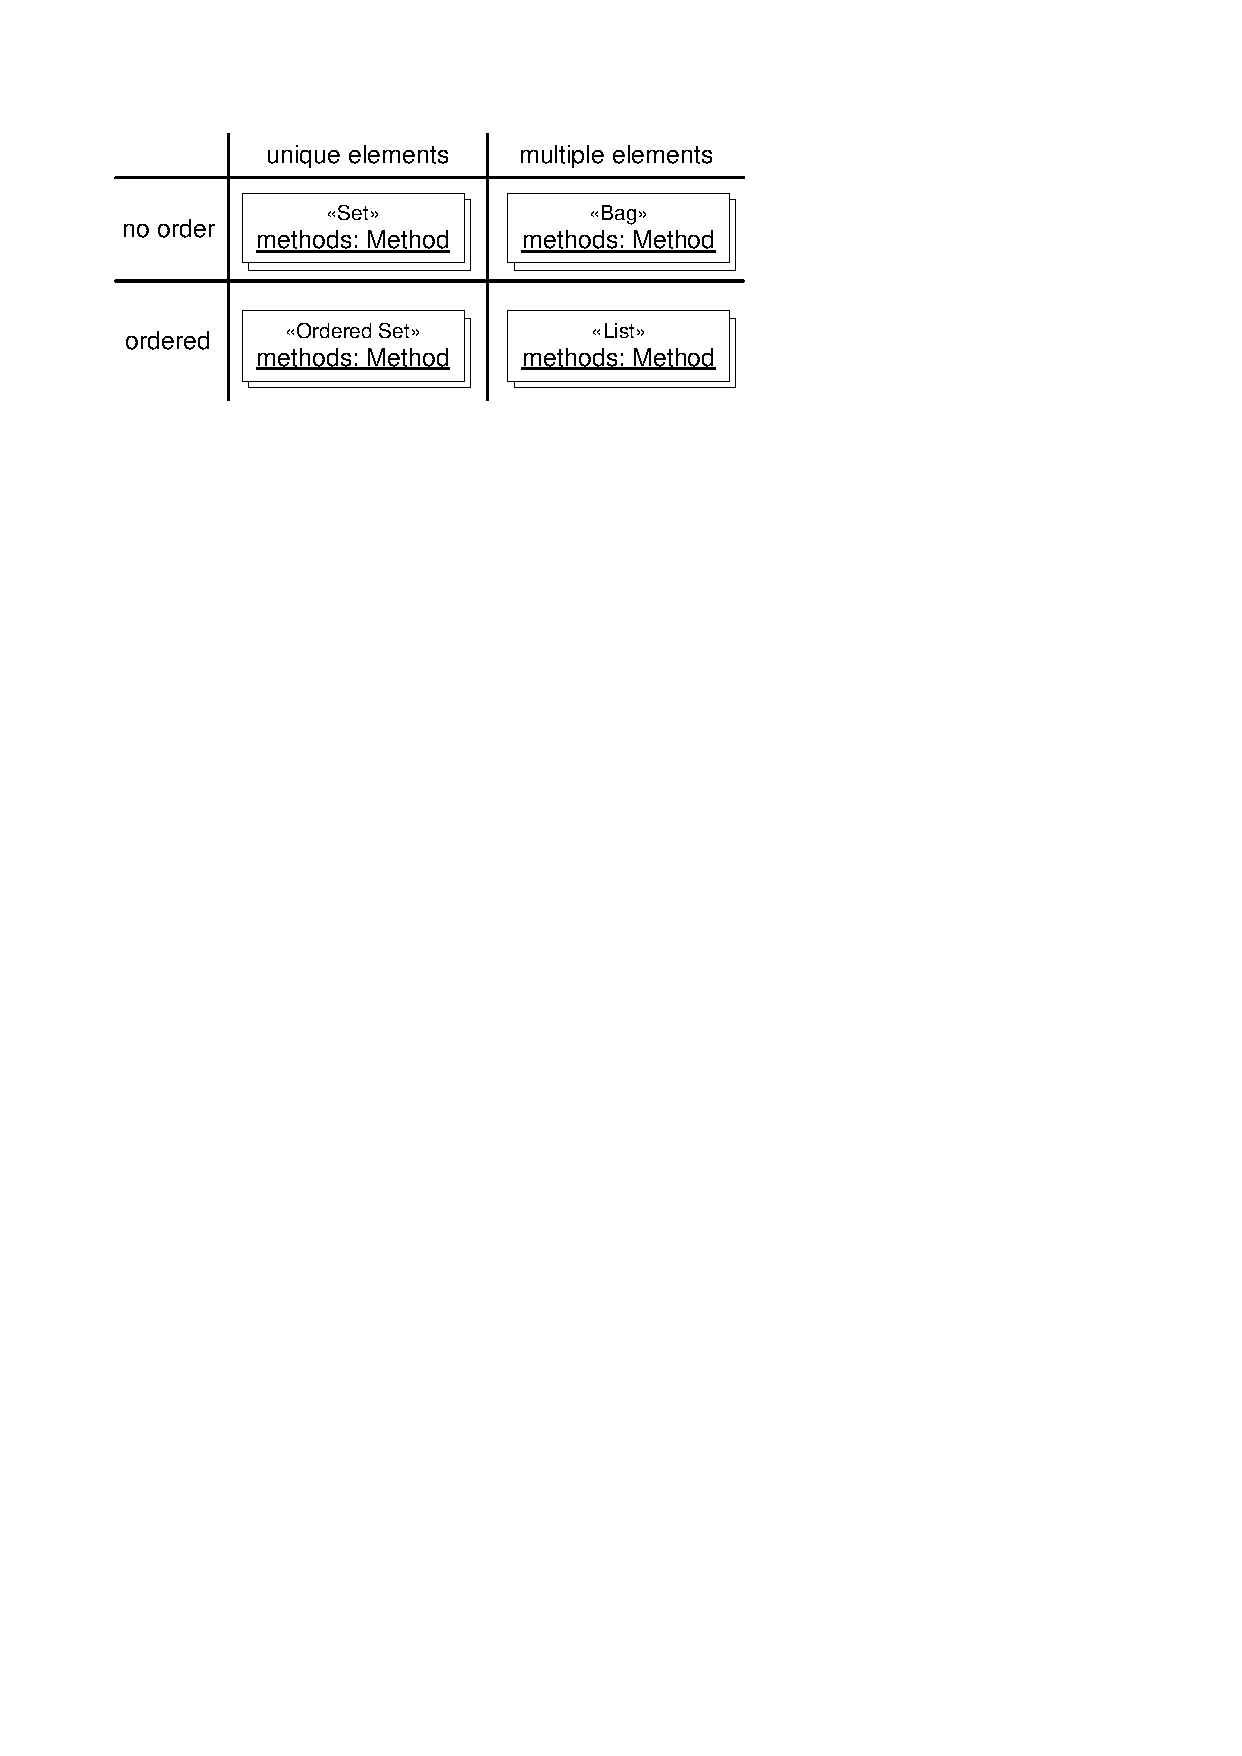
\includegraphics[scale=0.8]{figures/ObjectSets}
  \caption{Types of collection variables}
  \label{fig:ObjectSetsTypes}
\end{figure}

\tododt{We will only keep ordered sets and lists. Unordered sets and bags are omitted.}

\todomcp{explain collection variables and binding operators/states/semantics}

\todomcp{explain set size expressions (do we change the name?)}
\tododt{We should call the formerly known ObjectSetSizeExpression simply CollectionSizeExpression.}
\todomvd{According to the meeting on May, 25th, set size expressions are omitted in v0.2. We can use OCL instead.}

%\todomcp{If we bind an object set, can we use the bound object in other story
%pattern? E.g. to insert all elements bound by the object set into a container
%via a containment link?}
%\tododt{Yes, but I would use another concrete syntax (see
%Figures~\ref{fig:reuseObjSet1}, \ref{fig:InclusionLinksExample1}).}

%\begin{figure}[htb]
%		\centering
%		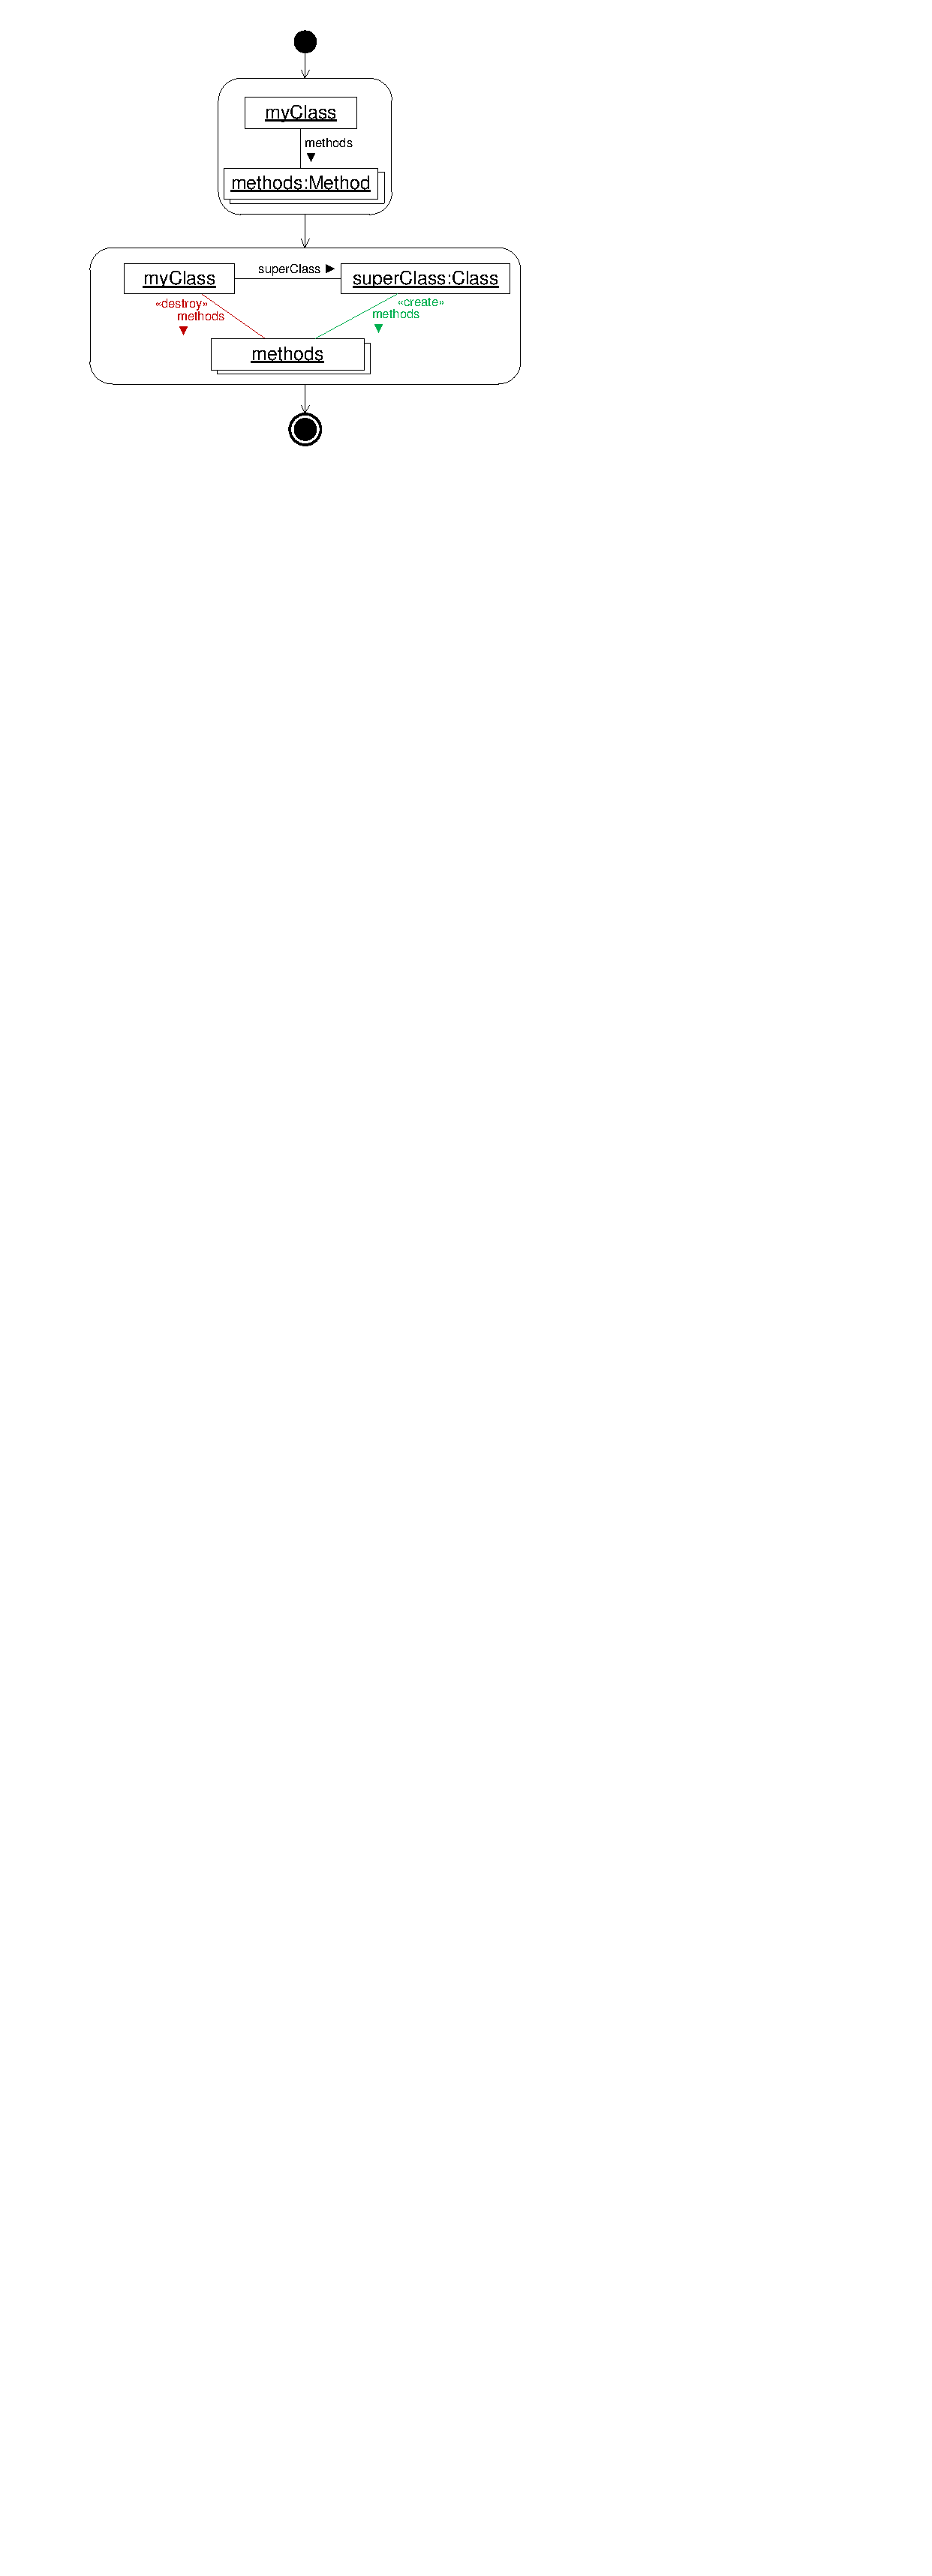
\includegraphics[scale=.8]{figures/ReuseObjectSet1}
%  	\caption{Reuse Objects in a Set}
%  	\label{fig:reuseObjSet1}
%\end{figure}

\todomcp{A collection variable contains no ObjectSetSizeExpression and no object is matched into the object set: collection variable is interpreted as optional and the matching succeeds.}
\tododt{We still should add an attribute to \fe{CollectionVariable} to distinguish the cases where at least one object should be matched or any number of objects including zero should be matched.
Stephan also wanted this expressiveness.}

\todomcp{All operators for comparison are allowed: <, <=, >, >=, = !=}

\begin{figure}[htb]
	%\begin{minipage}{.45\textwidth}
		\centering
		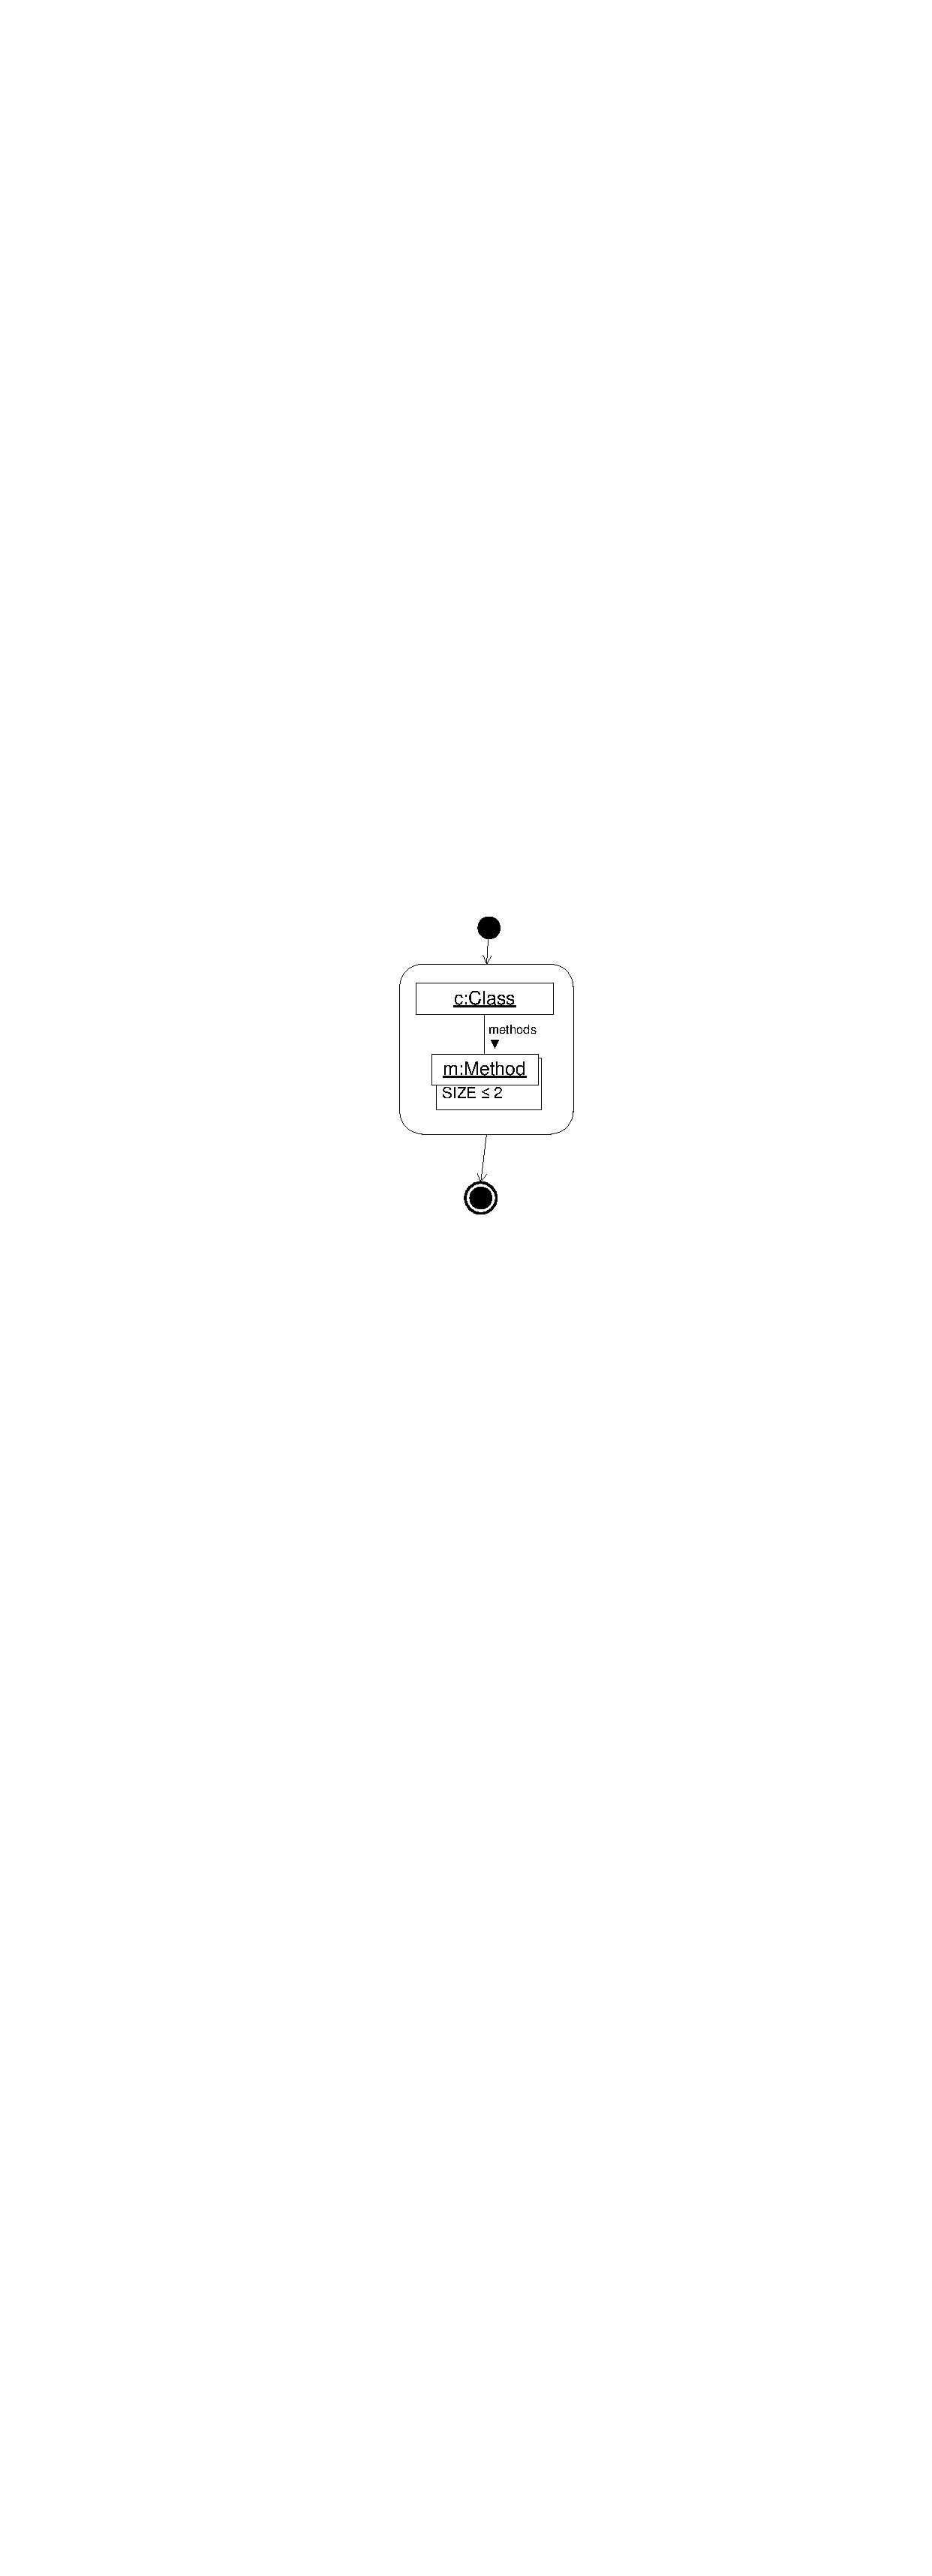
\includegraphics[scale=.7]{figures/ObjectSetSize}
  	\caption{Object Set Size}
  	\label{fig:objSetSize}
	%\end{minipage}
  %\hfill
  %\begin{minipage}{.45\textwidth}
  %	\centering
	%	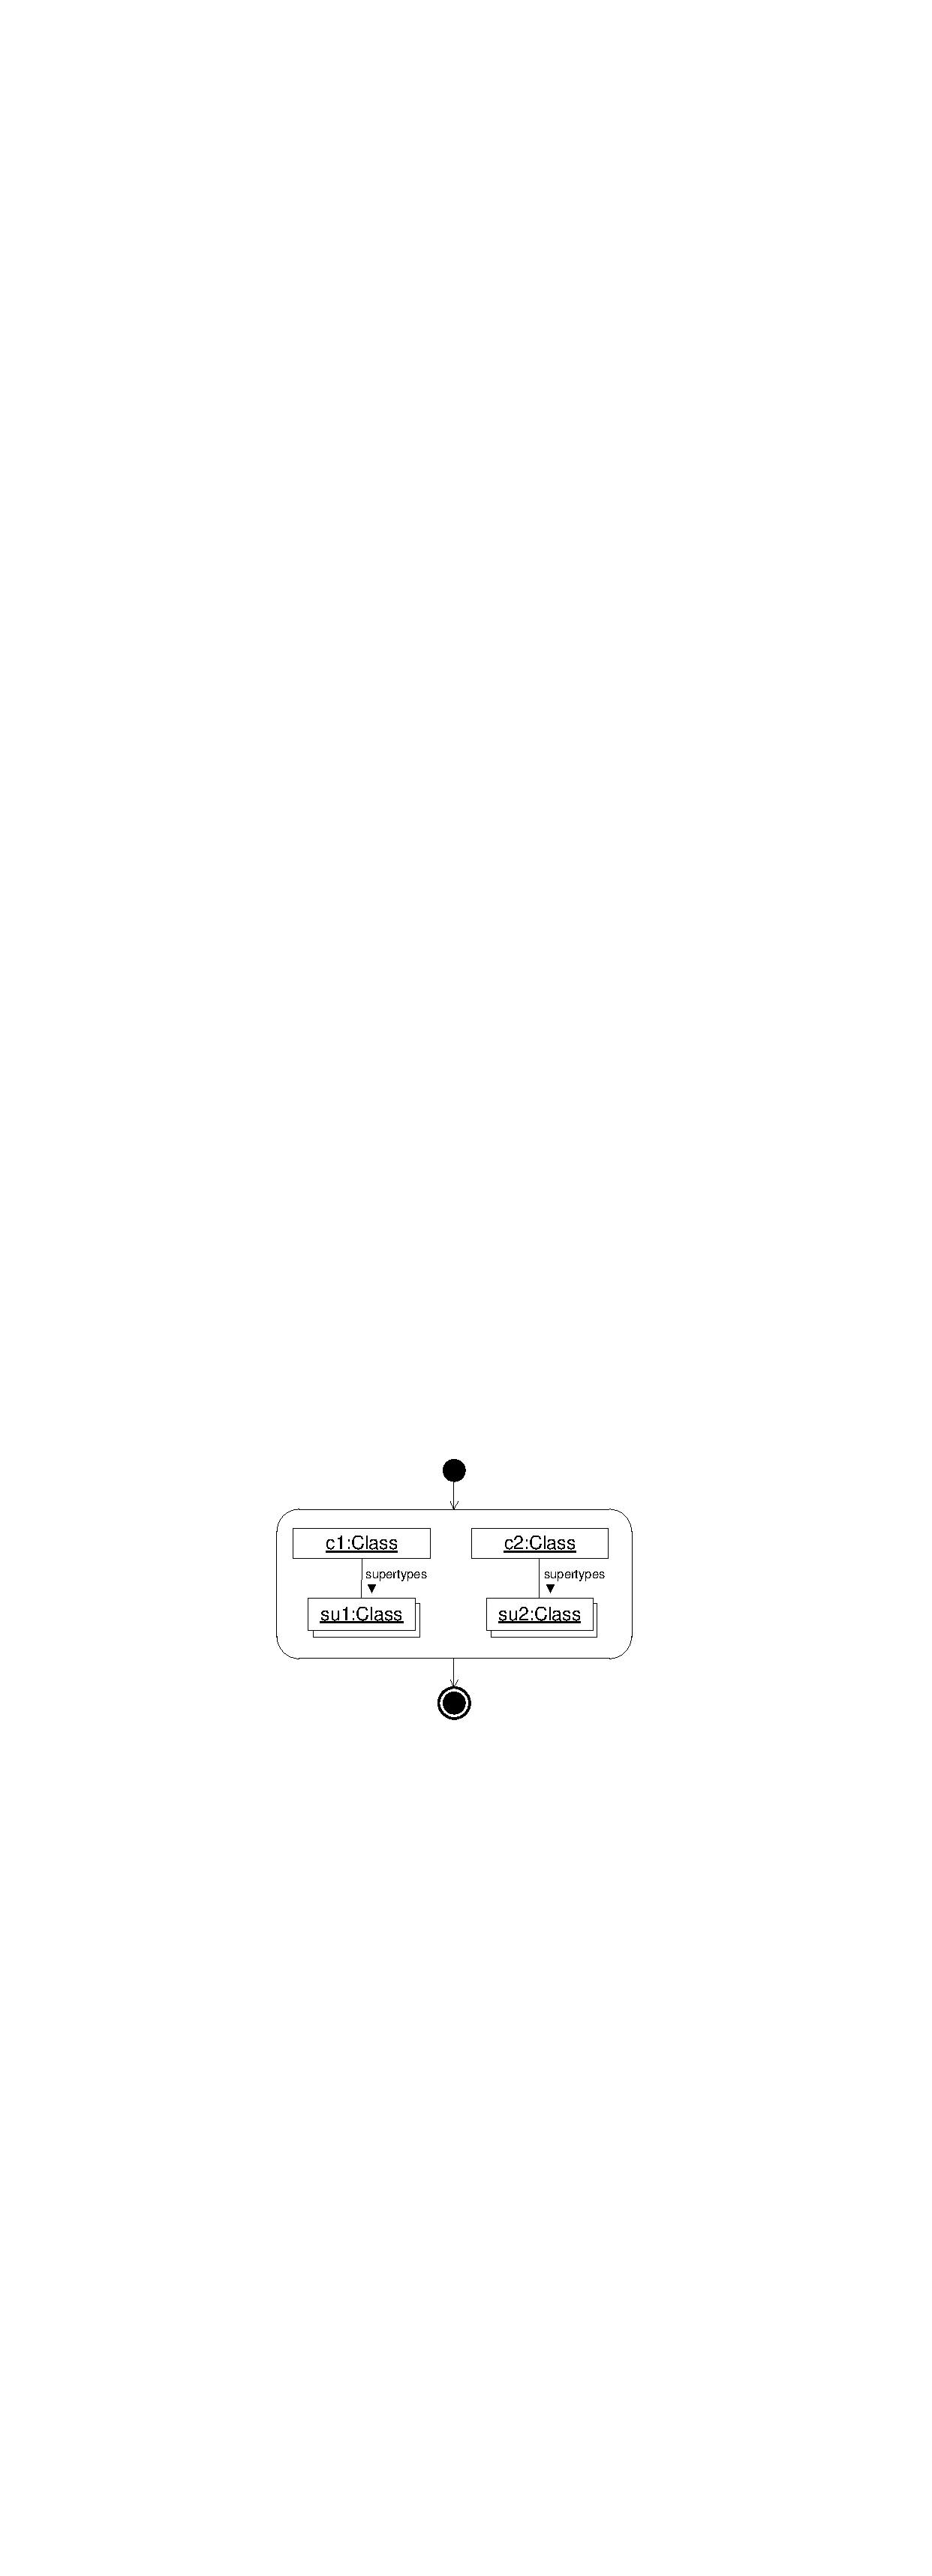
\includegraphics[scale=.8]{figures/IsomorphismInObjectSets}
  	%\caption{Isomorphism in Object Sets}
  	%\label{fig:isoObjSet}
	%\end{minipage}
\end{figure}

}%------ End of object set section

%\ext  %--- Comment this line to include pattern constraints into the document
{
\subsection{Pattern Constraints [CH]}

A pattern constraint defines an additional condition for a match that is evaluated and the end of the matching step, i.e., it is evaluated after all object and link variables have been matched. Since it is a condition, it needs to evaluate to true or false. If the pattern constraint is evaluated to true, then the match for the story pattern is valid. If the pattern constraint is evaluated to false, then the match is rejected.

A pattern constraint may use all object variables that are used in the same story pattern. Object variables are referred by their name. The pattern constraint may traverse the references of the objects bound to a particular object variable and access the attributes of the corresponding object. In the current version of story diagrams, we only support to use OCL for specifying pattern constraints. Then, the OCL constraint uses the name of the object variables to refer to objects and may use all features of OCL to access references and attributes of the corresponding objects.

\begin{figure}[htbp]
\center
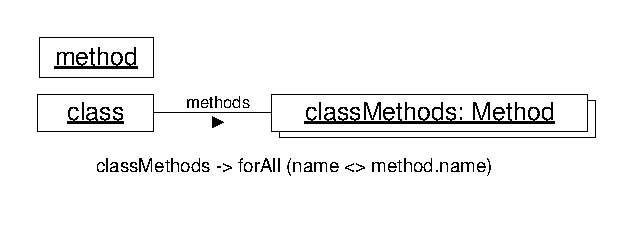
\includegraphics[width=0.6\columnwidth]{figures/PatternConstraint}
\caption{Example of a Pattern Constraint}
\label{fig:patternConstraint}
\end{figure}

Figure~\ref{fig:patternConstraint} gives an example for the concrete syntax of a pattern constraint. The story pattern has two bound object variables \fe{class} and \fe{method} of types \fe{GASTClass} and \fe{Method}, respectively. The pattern constraint is visualized as a label containing the OCL constraint. In the example, the OCL constraints specifies that all methods of \fe{class} need to have a name which is different from the name of \fe{method}. In addition, the story pattern matches all methods of \fe{class} in the object set \fe{classMethods}. The matching of the story pattern is successful only if the pattern constraint is fulfilled.

} %--- End of pattern constraints section


%\ext %--- Comment this line to include link constraints into the
{
\subsection{Link Constraints [CH]}
\label{sec:StoryPatterns:linkConstraints}

Link constraints specify constraints on the absolute position of an element in an ordered reference (\emph{link position constraints}, Section~\ref{sec:StoryPatterns:linkConstraints:posConstraint}) or on the position of an element relative to another element (\emph{link order constraints}, Section~\ref{sec:StoryPatterns:linkConstraints:orderConstraint}). These constraints are only applicable to link variables that are typed by ordered multi-valued references. All other kinds of links cannot be adorned with link constraints.

%\begin{itemize}
%  \item FIRST = matches the first element in the list, requires one link variable
%  \item LAST = matches the last element in the list, requires one link variable
%%  \item INDEX = matches the element at the specified index, requires one link variable
%%  \todoch{Our lowest index value is 0, not 1.}
%  \item DIRECT\_SUCCESSOR = requires two link variables, target of the second one must be located directly after the target of the first one in the list
%  \item SUCCESSOR = requires two link variables, target of the second one must be located somewhere after the target of the first one in the list
%\end{itemize}


\subsubsection{Link Position Constraints}
\label{sec:StoryPatterns:linkConstraints:posConstraint}

A link position constraint applies to a link variable that is typed by a multi-valued ordered reference. It specifies that the target object of the constrained link has to be the \emph{first} or the \emph{last} element in that reference. Other link position constraints are not supported. 

\todoch{Does anybody know a publication which explains the index constraint? In Alberts Habil, there are no index links.}
\tododt{Maybe you'll find it here: \cite{WW01_ag}. At least the link order constraints -- formerly known as multi links -- are described here including their concrete syntax.}
The \emph{index} link constraint which was available in earlier versions of story diagrams~\cite{•} is no longer supported. 
It was used to match an element which is located at a specific position in a multi-valued reference. 
However, that causes that upon creation of multiple elements it is not precisely defined where they are inserted into the list. 
In addition, the index may cause \emph{OutOfBounds} exceptions if the modeler specifies an invalid index.

Figure~\ref{fig:linkPositionConstraintFirst} shows an example of a link position constraint for matching the first element in a reference. The story pattern matches a \fe{FormalParameter} of the object which is bound to the object variable \fe{method}. The link position constraint \fe{\{first\}} specifies that the first \fe{FormalParameter} needs to be matched.

\begin{figure}[htbp]
\center
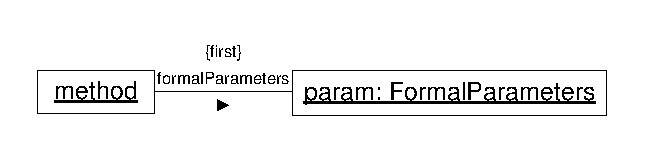
\includegraphics[width=0.75\columnwidth]{figures/LinkPositionConstraintFirst}
\caption{A \fe{\{first\}} link position constraint}
\label{fig:linkPositionConstraintFirst}
\end{figure}

Figure~\ref{fig:linkPositionConstraintLast} shows a similar story pattern which matches the last \fe{FormalParameter} instead of the first one. This is specified by the link position constraint \fe{\{last\}}.

\begin{figure}[htbp]
\center
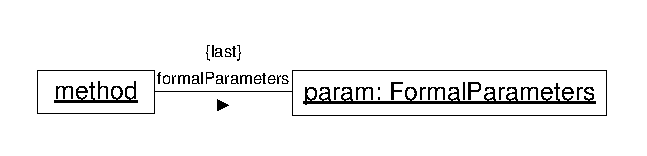
\includegraphics[width=0.75\columnwidth]{figures/LinkPositionConstraintLast}
\caption{A \fe{\{last\}} link position constraint}
\label{fig:linkPositionConstraintLast}
\end{figure}

If multiple link variables originate from the same object variable that refer to the same reference, only one of them may have a \fe{\{first\}} (or \fe{\{last\}}) link position constraint.

Link position constraints can be used with all feasible combinations of binding operators and binding semantics according to Table~\ref{tab:bindingCombinations_links}. For now, we discussed the semantics for using link position constraints for link variables with MANDATORY binding semantics and CHECK\_ONLY binding operator. If we use binding operator \create, the object is inserted at the specified position. If we use binding operator \destroy, the object is bound as described before and then deleted.

Figure~\ref{fig:linkPositionConstraintCreate} shows an example for using a link position constraint at a link variable with binding operator \create. The link position constraint causes the created \fe{FormalParameter} to be inserted at the last position of the \fe{formalParameters} of \fe{method}.

\begin{figure}[htbp]
\center
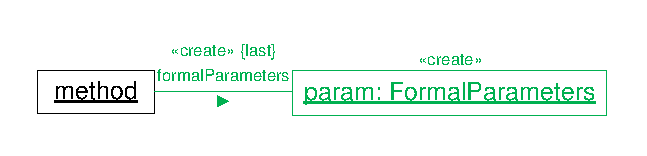
\includegraphics[width=0.75\columnwidth]{figures/LinkPositionConstraintCreate}
\caption{Link Position constraint at a created link.}
\label{fig:linkPositionConstraintCreate}
\end{figure}

If an OPTIONAL binding semantics is used, the matching will also be successful if no object at the specified position can be matched. Since we only restrict the position to the first or last position, this case will only apply if the link contains no objects at all. If the link variable additionally has binding operator \destroy, the object bound to the target object variable will be deleted. If the link variable additionally has binding operator \create, we have an optionally created link. If the link does not yet exist, it is created. The target element is inserted at the specified position in the reference. If the target element already exists in the reference but at a different position, the semantics of the optional create depends on the kind of the reference. If the reference requires objects to be unique in the reference, the target element is moved to the position specified by the optional create link variable. Otherwise, the element is added a second time at the specified position.

A combination with NEGATIVE binding semantics is also possible. If a link variable is negative and has a \fe{\{first\}} (or \fe{\{last\}}) link position constraint, then the object bound to the target object variable must not be the first (or last) object in the corresponding reference. That means, we negate the link position constraint rather than the whole link variable which causes a slight change of the NEGATIVE binding semantics of link variables.

%\todoch{How is the semantics of link position constraints on negative links as shown in Figure~\ref{fig:linkPositionConstraintNegative}? Two alternatives: 1) The target object is not the first (or last) element in the reference. That means we negate the link position constraint and not the whole link variable. 2) There exists no link pointing to the first (or last) element. That means we negate the whole link which in turn means that there is no element in the reference and the link position constraint has no effect. I prefer 1) even though it slightly changes the semantics of the negative binding semantics (because it is applied to the link constraint rather than the link itself).}

Figure~\ref{fig:linkPositionConstraintNegative} shows an example for a negative link with a link position constraint. The \fe{FormalParameter} which is bound to \fe{param} must not be the first \fe{formalParameter} of the method which is bound to \fe{method}.


\begin{figure}[htbp]
\center
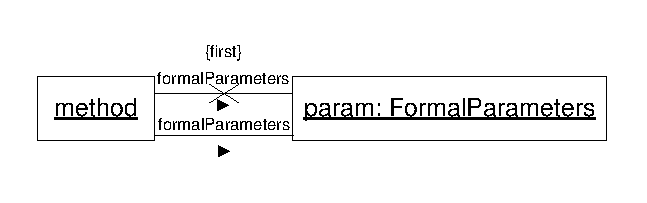
\includegraphics[width=0.75\columnwidth]{figures/LinkPositionConstraintNegated}
\caption{A negative link with a \fe{\{first\}} link position constraint}
\label{fig:linkPositionConstraintNegative}
\end{figure}



\subsubsection{Link Order Constraints}
\label{sec:StoryPatterns:linkConstraints:orderConstraint}

Link order constraints specify a relative order between two objects in a multi-valued ordered reference. A link order constraint therefore connects two link variables which we denote as the source link variable and target link variable of the link order constraint. Then, the object matched via the target link variable must either be the \emph{direct successor} or an  \emph{arbitrary successor} of the object matched via the source link variable.

Figure~\ref{fig:linkOrderConstraintDirectSuccessor} shows an example of a link order constraint requiring to match two subsequent \fe{FormalParameters} of \fe{method}. Therefore, the two link variables from \fe{method} to \fe{param1} and \fe{param2} are connected by a link order constraint \fe{\{next\}}. Then, the object matched to \fe{param2} must be a direct successor of the object matched to \fe{param1}.

\begin{figure}[htbp]
\center
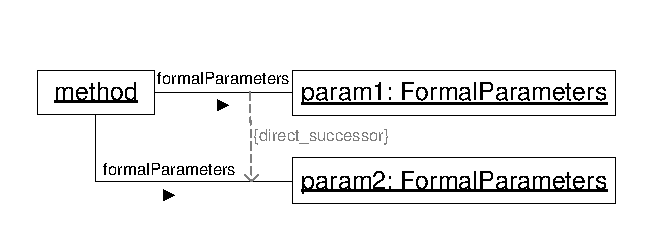
\includegraphics[width=0.75\columnwidth]{figures/LinkOrderConstraintDirectSuccessor}
\caption{A link order constraint specifying a \fe{\{direct\_successor\}}.}
\label{fig:linkOrderConstraintDirectSuccessor}
\end{figure}

Figure~\ref{fig:linkOrderConstraintSuccessor} shows an example of a link order constraint requiring to match two \fe{FormalParameters} of \fe{method} where one succeeds the other. Therefore, the two link variables from \fe{method} to \fe{param1} and \fe{param2} are connected by a link order constraint \fe{\{successor\}}. Then, the object matched to \fe{param2} must be an arbitrary successor of the object matched to \fe{param1}. The matching of the successor is non-deterministic. Thus, a matching retrieved for the story pattern in Figure~\ref{fig:linkOrderConstraintDirectSuccessor} is a valid matching for the story pattern in Figure~\ref{fig:linkOrderConstraintSuccessor} as well. A matching retrieved for the story pattern in Figure~\ref{fig:linkOrderConstraintSuccessor}, however, will not be a valid matching for the story pattern in Figure~\ref{fig:linkOrderConstraintDirectSuccessor} in the general case.

\begin{figure}[htbp]
\center
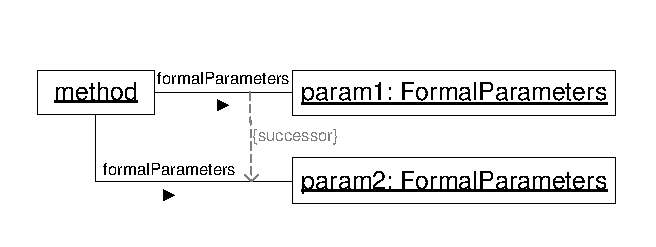
\includegraphics[width=0.75\columnwidth]{figures/LinkOrderConstraintSuccessor}
\caption{A link order constraint specifying a \fe{\{successor\}}.}
\label{fig:linkOrderConstraintSuccessor}
\end{figure}

Link order constraints can be applied to links that have a binding operator \create or \destroy. In case of \destroy, the matching is carried out as described before. In case of \create, links corresponding to the link variables are created in the instance model. The target objects are then inserted into the reference at the specified positions. If the source link variable (or target link variable) of the link order constraint has a \create binding operator, then the object is inserted directly before (or after) the object bound via the target (or source) link variable. We also apply this semantics if the link order constraint requires the objects only to be indirect successors to avoid non-determinism.

\begin{figure}[htbp]
\center
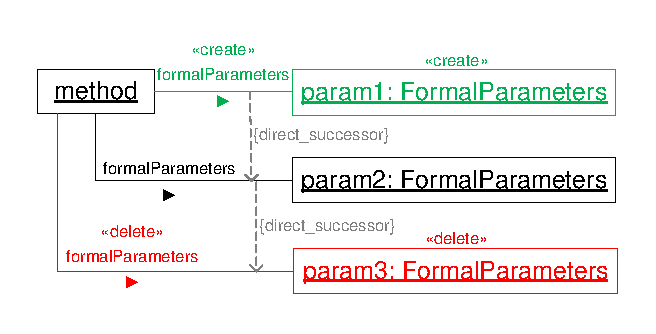
\includegraphics[width=0.75\columnwidth]{figures/LinkOrderConstraintDirectSuccessorCreateDelete}
\caption{Using link order constraints with binding operators \create and \destroy.}
\label{fig:linkOrderConstraintDirectSuccessorCreateDelete}
\end{figure}

Figure~\ref{fig:linkOrderConstraintDirectSuccessorCreateDelete} shows an example for using link order constraints with the binding operators \create and \destroy. The story pattern matches two successive \fe{FormalParameters} of \fe{method} and binds them to the object variables \fe{param2} and \fe{param3}. If the matching was successful, the parameter bound to \fe{param3} is deleted and removed for the reference. Then, a new \fe{FormalParameter} is created and inserted directly before \fe{param2}.

If a link variable with binding operator \create is the target link variable (or source link variable) of several \emph{indirect successor} link order constraints, then after target object of the link variable is inserted directly behind (or before) the object with the highest index. If  multiple link constraints are applied to the same link variable with binding operator \create, enforcing the right-hand side of the story pattern may fail if the link constraints are unsatisfiable for the reference.

If both, the source link variable and the target link variable of the link order constraint, carry a binding operator, both need to carry the same binding operator. If one link variable has a binding operator \create and the other one has \destroy, then the reference for inserting the new object has been deleted before the object can be inserted. Since the semantics in undefined in that case, we forbid this case.

Link order constraints can be used in combination with an optional binding semantics of the source or target link variable. In case the link variable carries no binding operator or binding operator \destroy, the matching process is performed as described before. If no matching for the optional link variables satisfying the link order constraints can be found, the matching does not fail. If the a link variable carries an optional create, the semantics depends on the kind of reference. If the reference does not contain the object bound to the target link variable, it is added according to the link order constraint. If the reference already contains the target object, but at a position which does not satisfy the link order constraint, then there are two possibilities.  If the reference requires objects to be unique in the reference, the target element is moved to a position specified by the link order constraints. Otherwise, the element is added a second time at a position specified by the link order constraints. In both cases, the rules for inserting an object into a reference as described above for non-optional link variables are applied.

Link order constraints may also be used in combination with a negative binding semantics of the source or target link variable. If a negative link variable is the target link variable of a \emph{direct successor} (or \emph{indirect successor}) link order constraint, then the target object must not be located directly after (of indirectly after) the object bound to the source link variable. If a negative link variable is the source link variable of a \emph{direct successor} (or \emph{indirect successor}) link order constraint, then the target object must not be located directly before (of indirectly before) the object bound to the target link variable. That means, we negate the link order constraint rather than the whole link variable if the link variable is the source or target link variable of a link order constraint. That causes a slight change in the definition of the negative binding semantics for link variables.

\begin{figure}[htbp]
\center
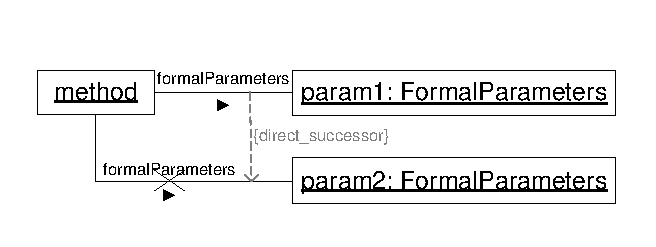
\includegraphics[width=0.75\columnwidth]{figures/LinkOrderConstraintDirectSuccessorNegative}
\caption{A link order constraint with a negative link.}
\label{fig:linkOrderConstraintDirectSuccessorNegative}
\end{figure}

Figure~\ref{fig:linkOrderConstraintDirectSuccessorNegative} shows an example of a negative link variable which is the target link variable of a \emph{direct successor} link order constraint. In the example, two \fe{FormalParameters} of \fe{method} are to be matched. The object bound to \fe{param1} may be an arbitrary \fe{FormalParameter}. The object variable \fe{param2} may be matched to any \fe{FormalParameter} of \fe{method} except for the \fe{FormalParameter} that is directly located behind the object bound to \fe{param1}.

It is possible to use multiple link order constraints on a negative link. Then, all of the specified conditions need to hold. However, for each link order constraint either the source link variable or the target link variable may be negative, but not both.

\begin{figure}[htbp]
\center
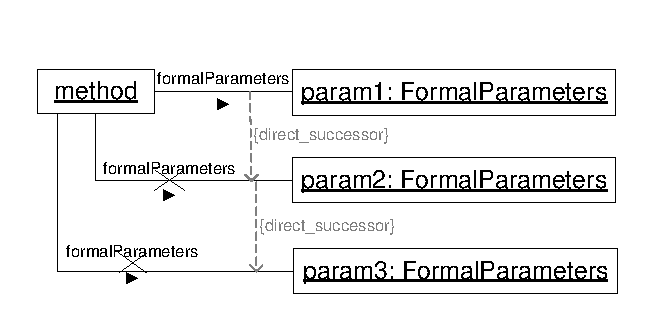
\includegraphics[width=0.75\columnwidth]{figures/LinkOrderConstraintDirectSuccessorNegative2}
\caption{Applying Multiple Link Order Constraints on a Negative Link Variable}
\label{fig:linkOrderConstraintDirectSuccessorNegative2}
\end{figure}

Figure~\ref{fig:linkOrderConstraintDirectSuccessorNegative2} shows an example of applying multiple link order constraint to a negative link variable. The story pattern matches three \fe{FormalParameters} of \fe{method}. The matching must fulfill the following conditions which are implied by the negative link variable from \fe{method} to \fe{param2} and the two link order constraints: \fe{param2} must not be an indirect successor of \fe{param1} and \fe{param3} must not be the direct successor of \fe{param2}. If only one of the two conditions is not fulfilled, then the story pattern does not match.

\begin{figure}[htbp]
\center
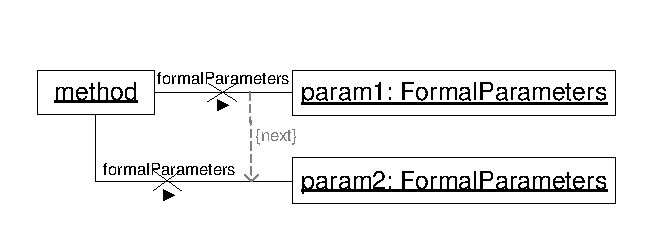
\includegraphics[width=0.75\columnwidth]{figures/LinkOrderConstraintDirectSuccessorNegative3}
\caption{Invalid Combination of Link Order Constraints and Negative Link Variables.}
\label{fig:linkOrderConstraintDirectSuccessorNegative3}
\end{figure}

Figure~\ref{fig:linkOrderConstraintDirectSuccessorNegative3} shows an example of an invalid combination of negative link variables and link order constraints because both, the source and the target link variable of the link order constraint, are negative. 

Link order constraints may not form circles or unsatisfiable story patterns. An example of an unsatisfiable story pattern is given by Figure~\ref{fig:linkConstraintUnsatisfiablePattern}. In this story pattern, the object bound to \fe{param2} must be the first \fe{FormalParameter} of \fe{method}. At the same time, the link order constraint requires the object bound to \fe{param2} to be the direct successor of the object bound to \fe{param1}. Since this is not possible, the pattern is unsatisfiable and will never match.

\tododt{Should we refer to \cite{TMG06} and explain if or how we solve the issues discussed there in Section 3.1.3 (see Figure~2)?}

\begin{figure}[htbp]
\center
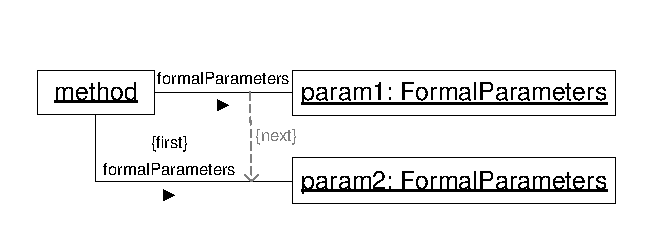
\includegraphics[width=0.75\columnwidth]{figures/LinkConstraintUnsatisfiablePattern}
\caption{Link Constraints causing a Story Pattern to be unsatisfiable.}
\label{fig:linkConstraintUnsatisfiablePattern}
\end{figure}

} %--- End of link constraint subsection

\subsection{Maybe Links [CH]}
\label{sec:StoryPatterns:specialLinks:maybeLink}

Story patterns are matched by using isomorphic matchings. That means that two object variables in a story pattern may not be matched to the same object of the instance model. A matching which matches two object variables to the same object is, thus, considered to be invalid. In some situations, however, such matchings should be explicitly allowed. Then, the isomorphic matching must be disabled. This may be achieved by connecting the object variables with a maybe link. Figure \ref{fig:maybeLink} shows the concrete syntax of maybe links. 

\tododt{Please clarify the semantics of a \emph{maybe} link.
It allows two object variables to be matched to the same object.
For all aother variables an isomorphic matching is performed.
I would also emphasize \emph{maybe}.}

\begin{figure}[htb]
  \centering
  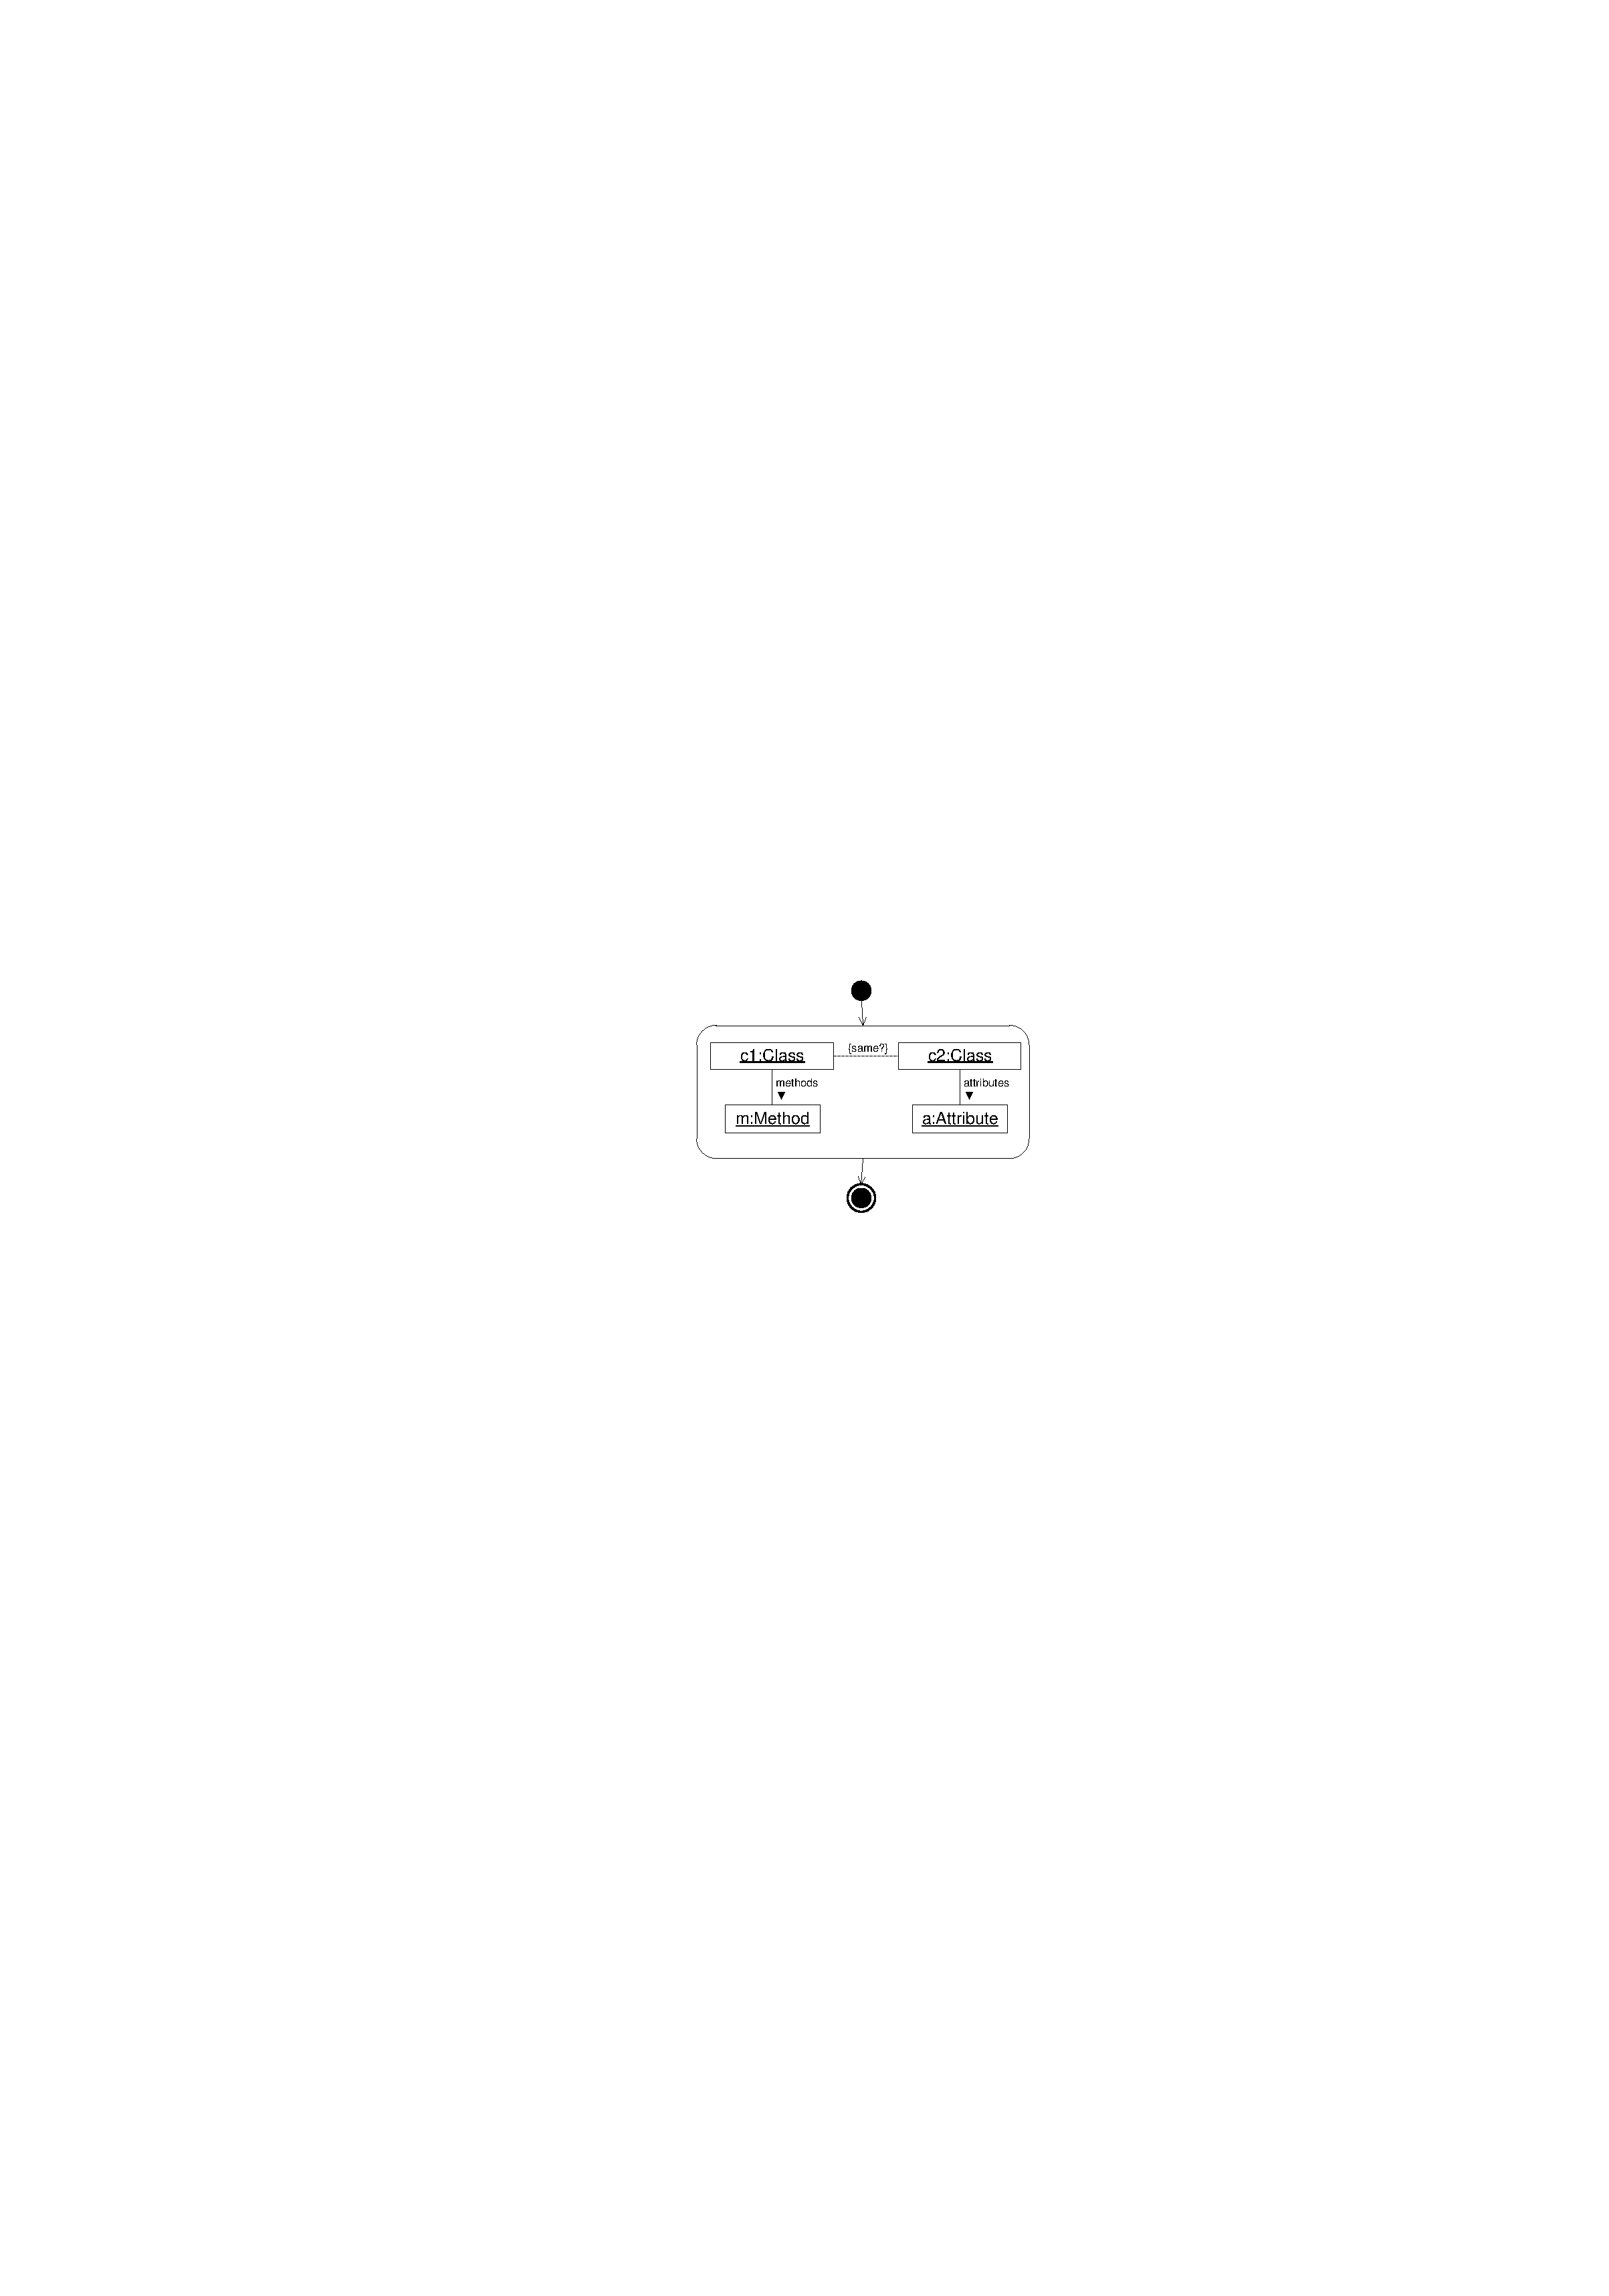
\includegraphics[scale=.8]{figures/MaybeLink}
  \caption{Maybe Link allowing two Object Variables to be matched to the same Object}
  \label{fig:maybeLink}
\end{figure}

If two object variables are connected by a maybe link, they both must be mandatory or optional. In addition, a maybe link requires the object variables to be matched or destroyed, but not created.  



\subsection{Inclusion Links [DT]}
\label{sec:StoryPatterns:inclusion}

There are cases when you want to add additional objects to a set of objects matched to a collection variable as described in Section~\ref{sec:StoryPatterns:objectsets}.
Since a collection variable does not explicitly represent a collection object in the sense of Java\footnote{
We do not expliciltly model collection objects in story diagrams.
The type of a collection variable is that of the contained objects and not the type of a collection object like \texttt{java.util.Collection}.},
we need a way to describe the addition or removal of objects to or from such an object collection as well as checking if an object is included in an object collection.
We introduce \emph{inclusion links} for this purpose.

\begin{figure}[htb]
	\begin{minipage}{.43\textwidth}
		\centering
		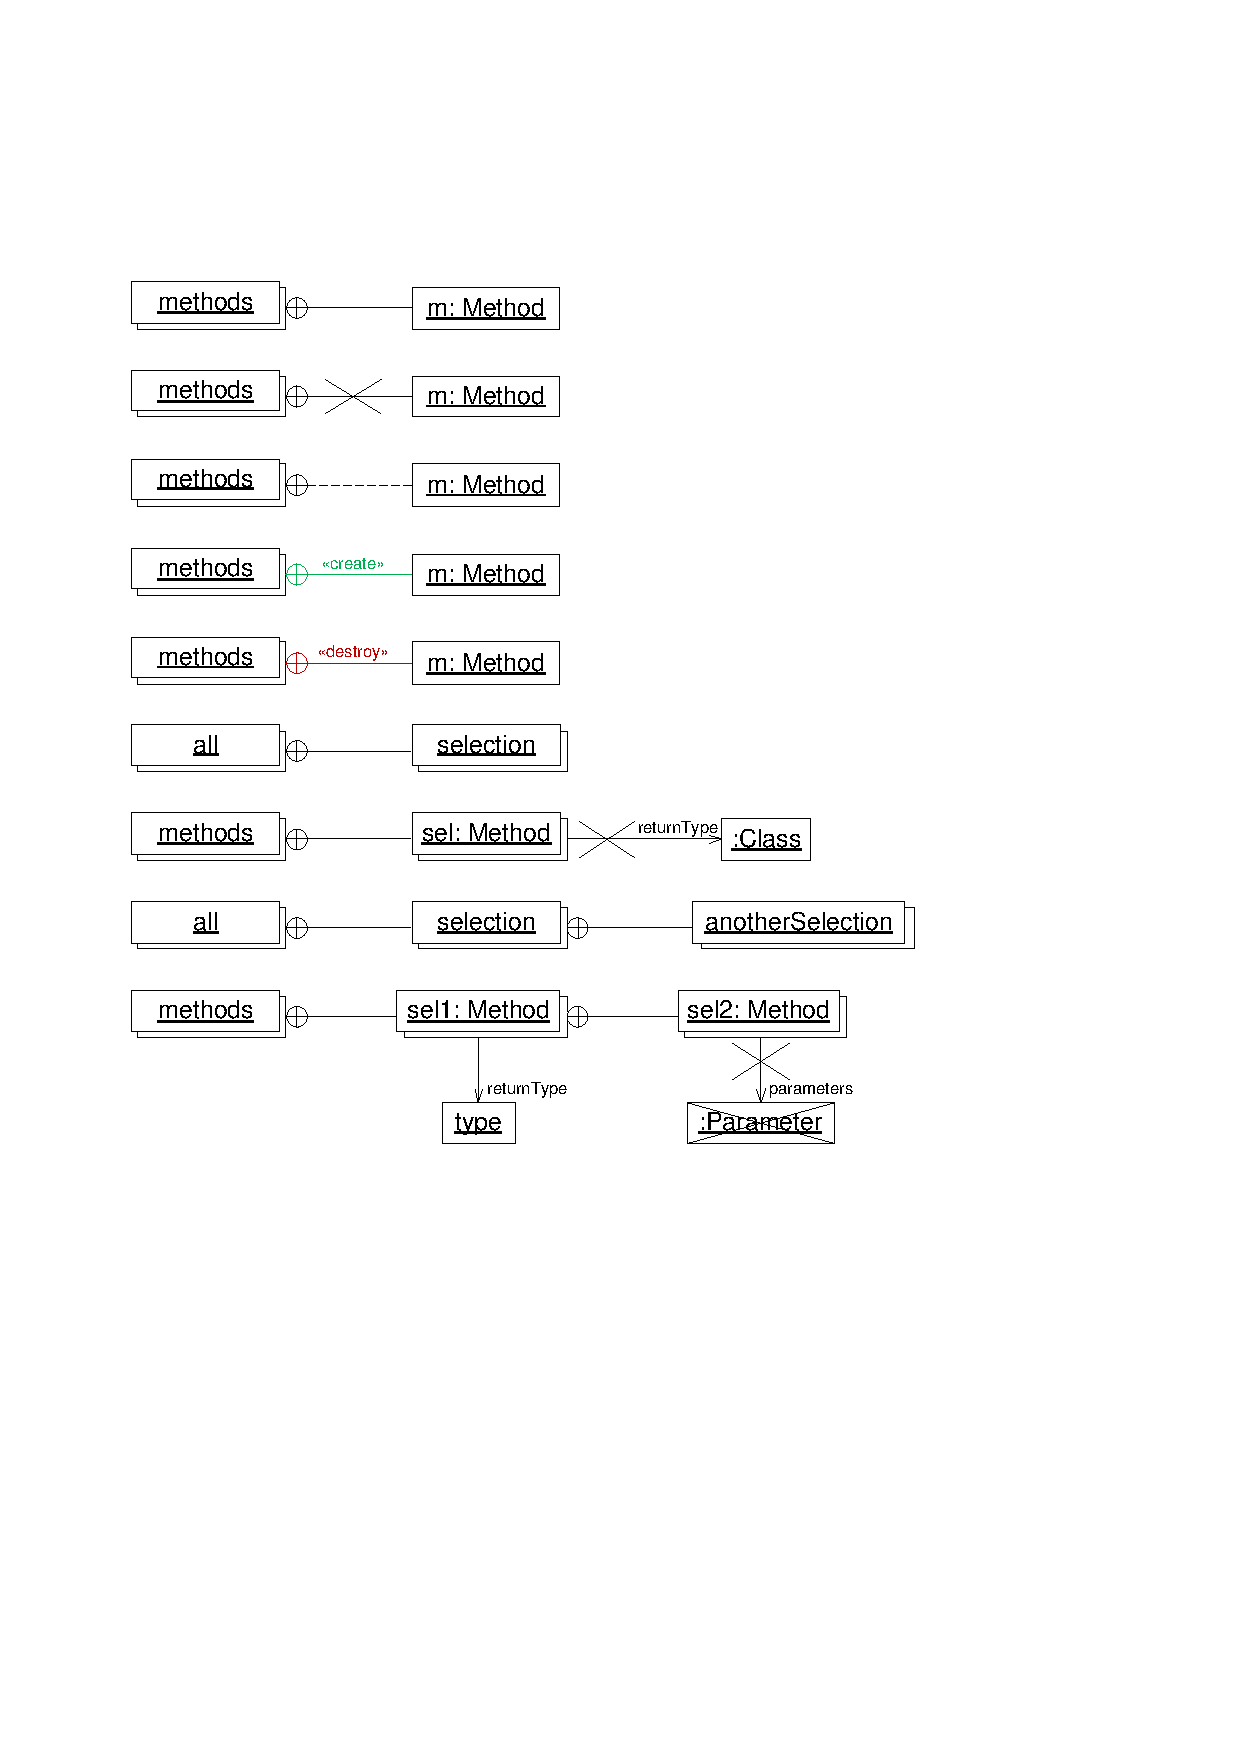
\includegraphics[width=\linewidth]{figures/InclusionLinks}
    \caption{Notation of Inclusion Links}
    \label{fig:InlucionLinks}
	\end{minipage}
  \hfill
  \begin{minipage}{.47\textwidth}
  	\centering
		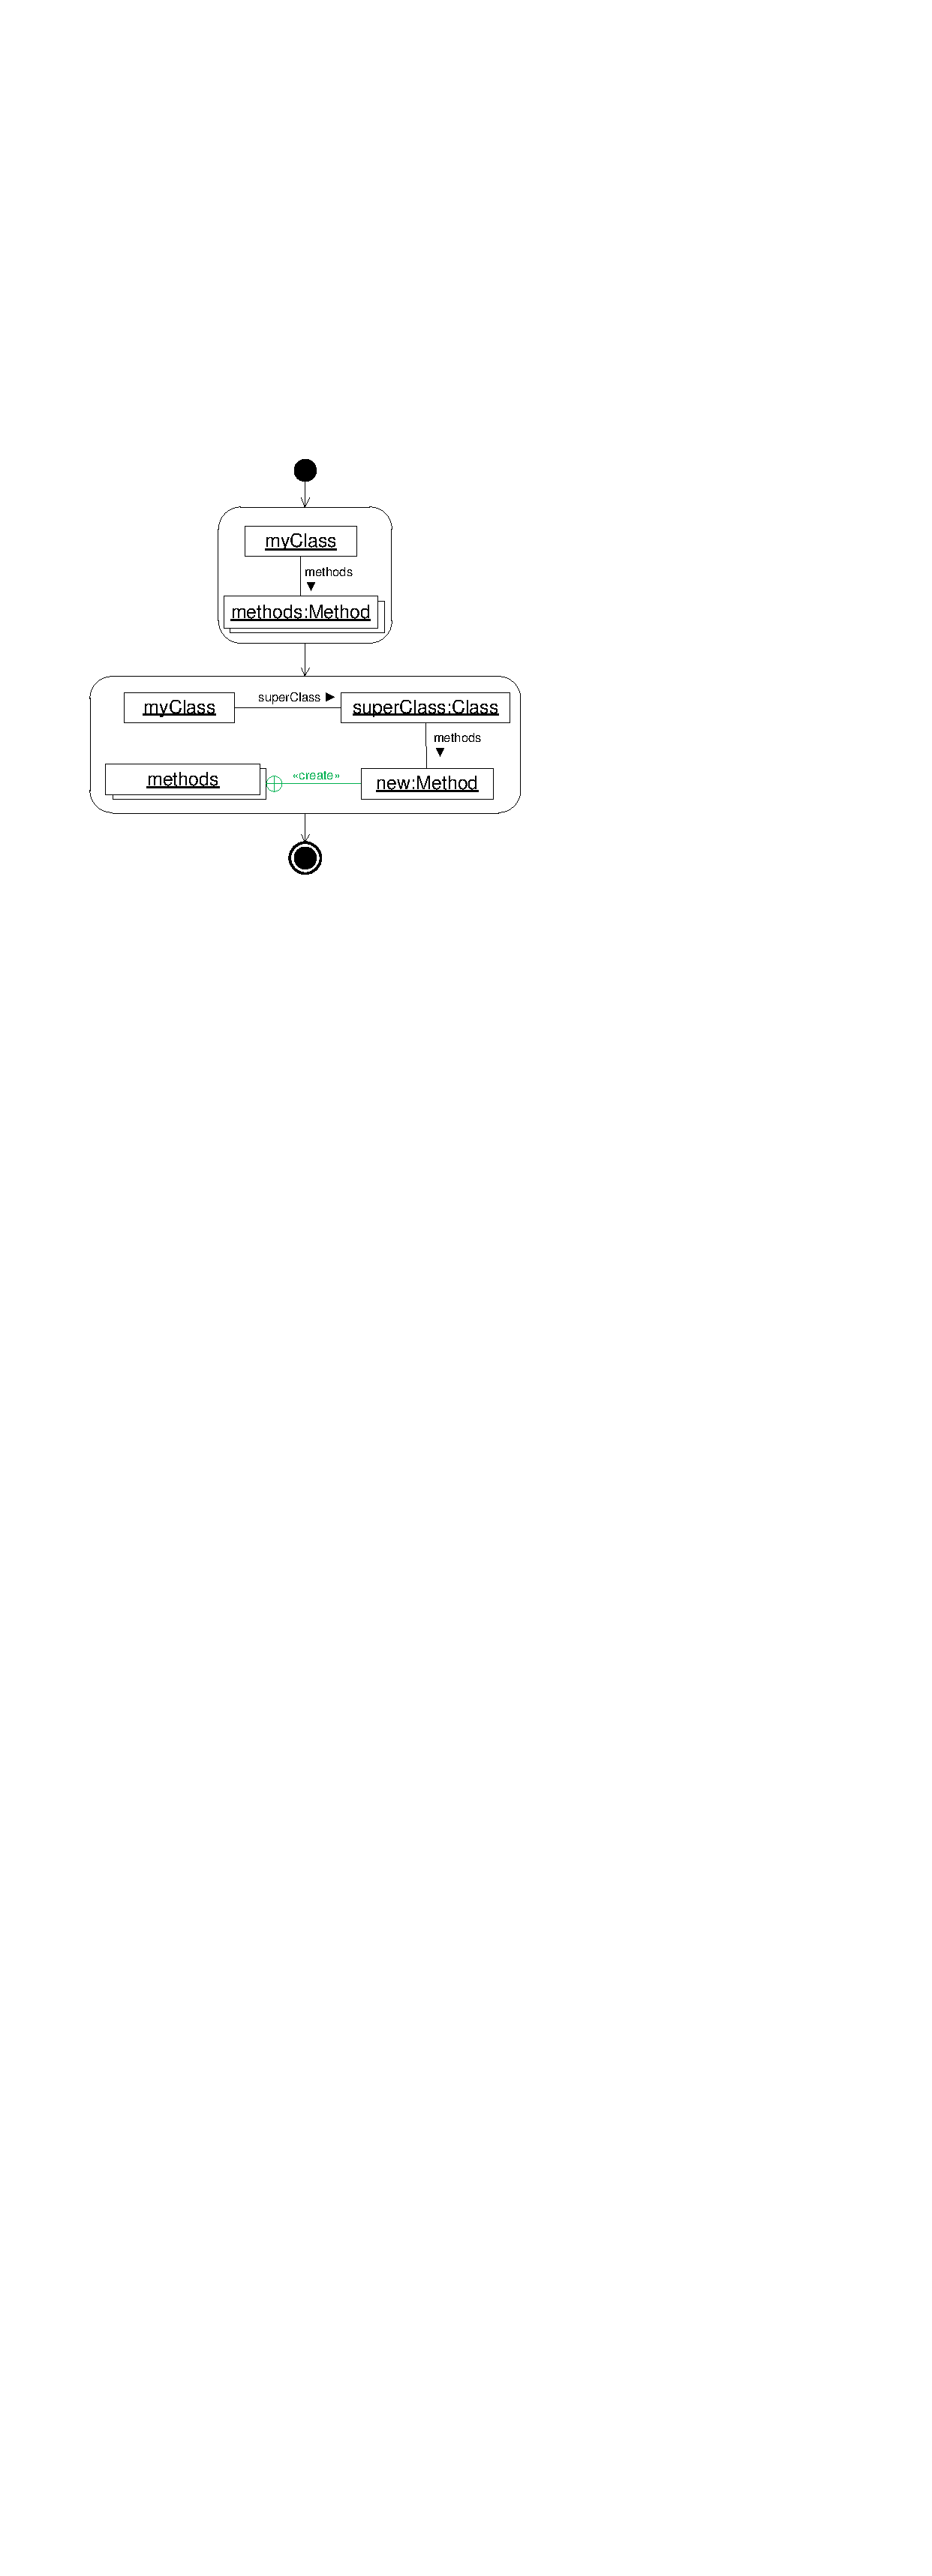
\includegraphics[width=\linewidth]{figures/InclusionLinksExample1}
    \caption{Add an Object to a Collection}
    \label{fig:InclusionLinksExample1}
	\end{minipage}
\end{figure}

An inclusion link represents a containment relation between two variables in a story pattern.
It can always be used between a collection variable and another variable to specify that
an object (or a set of objects) represented by a variable is contained in an object set represented by a collection variable.
An inclusion link is represented by a line between a collection variable and another object
variable as illustrated in Figure~\ref{fig:InlucionLinks}~a).
The circle containing a plus determines which of the two sides of the link is containing the other one.
In Figure~\ref{fig:InlucionLinks}~a), the collection \fe{methods} contains an object \fe{aMethod}.

In contrast to link variables that are typed over an association, inclusion links are not typed at all.
They only represent a containment of an object in a collection of objects.
But similar to link variables, this relation can be checked to be existent between a collection and an object
or be used to match new objects.
While the pattern in Figure~\ref{fig:InlucionLinks} a) specifies to check if the object \fe{aMethod} is contained in the collection \fe{methods},
the pattern in Figure~\ref{fig:InlucionLinks} b) specifies to match a \fe{Method} object which is contained in the collection \fe{methods}.

Similar to other links, inclusion links can be used with bound, unbound, or maybe-bound object variables, can be negative or optional, use
\create\ or \destroy\ stereotypes (see Figure~\ref{fig:InlucionLinks} a) to f)).
Case c) in Figure~\ref{fig:InlucionLinks} defines that the matching is only successful if no \fe{Method} object can be found in the \fe{methods} collection.
Accordingly, case d) specifies to optionally match a \fe{Method} object contained in the \fe{methods} collection
(see the description of binding semantics in Section~\ref{sec:StoryPatterns:binding:semantics} for details).
Case e) specifies to create an inclusion relation between the object \fe{aMethod} and the collection \fe{methods},
i.e.\ to add the object \fe{aMethod} to the collection \fe{methods}.
Analogously, case f) specifies to remove the object \fe{aMethod} from the collection \fe{methods}.
Furthermore, inclusion links can also be used between two collection variables as illustrated in Figure~\ref{fig:InlucionLinks} f)
to check if all objects in the collection \fe{selection} are contained in the collection \fe{all}.

By means of inclusion links, a collection variable that has been matched to a set of objects
can be modified afterwards by adding or removing objects.
Using story diagrams as described in Section~\ref{sec:StoryDiagrams},
one can, for example, collect a set of \fe{Method} objects in a collection \fe{methods}
as illustrated in the first story node in Figure~\ref{fig:InclusionLinksExample1}
and then add another \fe{Method} object to the same collection in a following story node that reuses the previously matched set of objects.

\begin{figure}[htb]
  \centering
  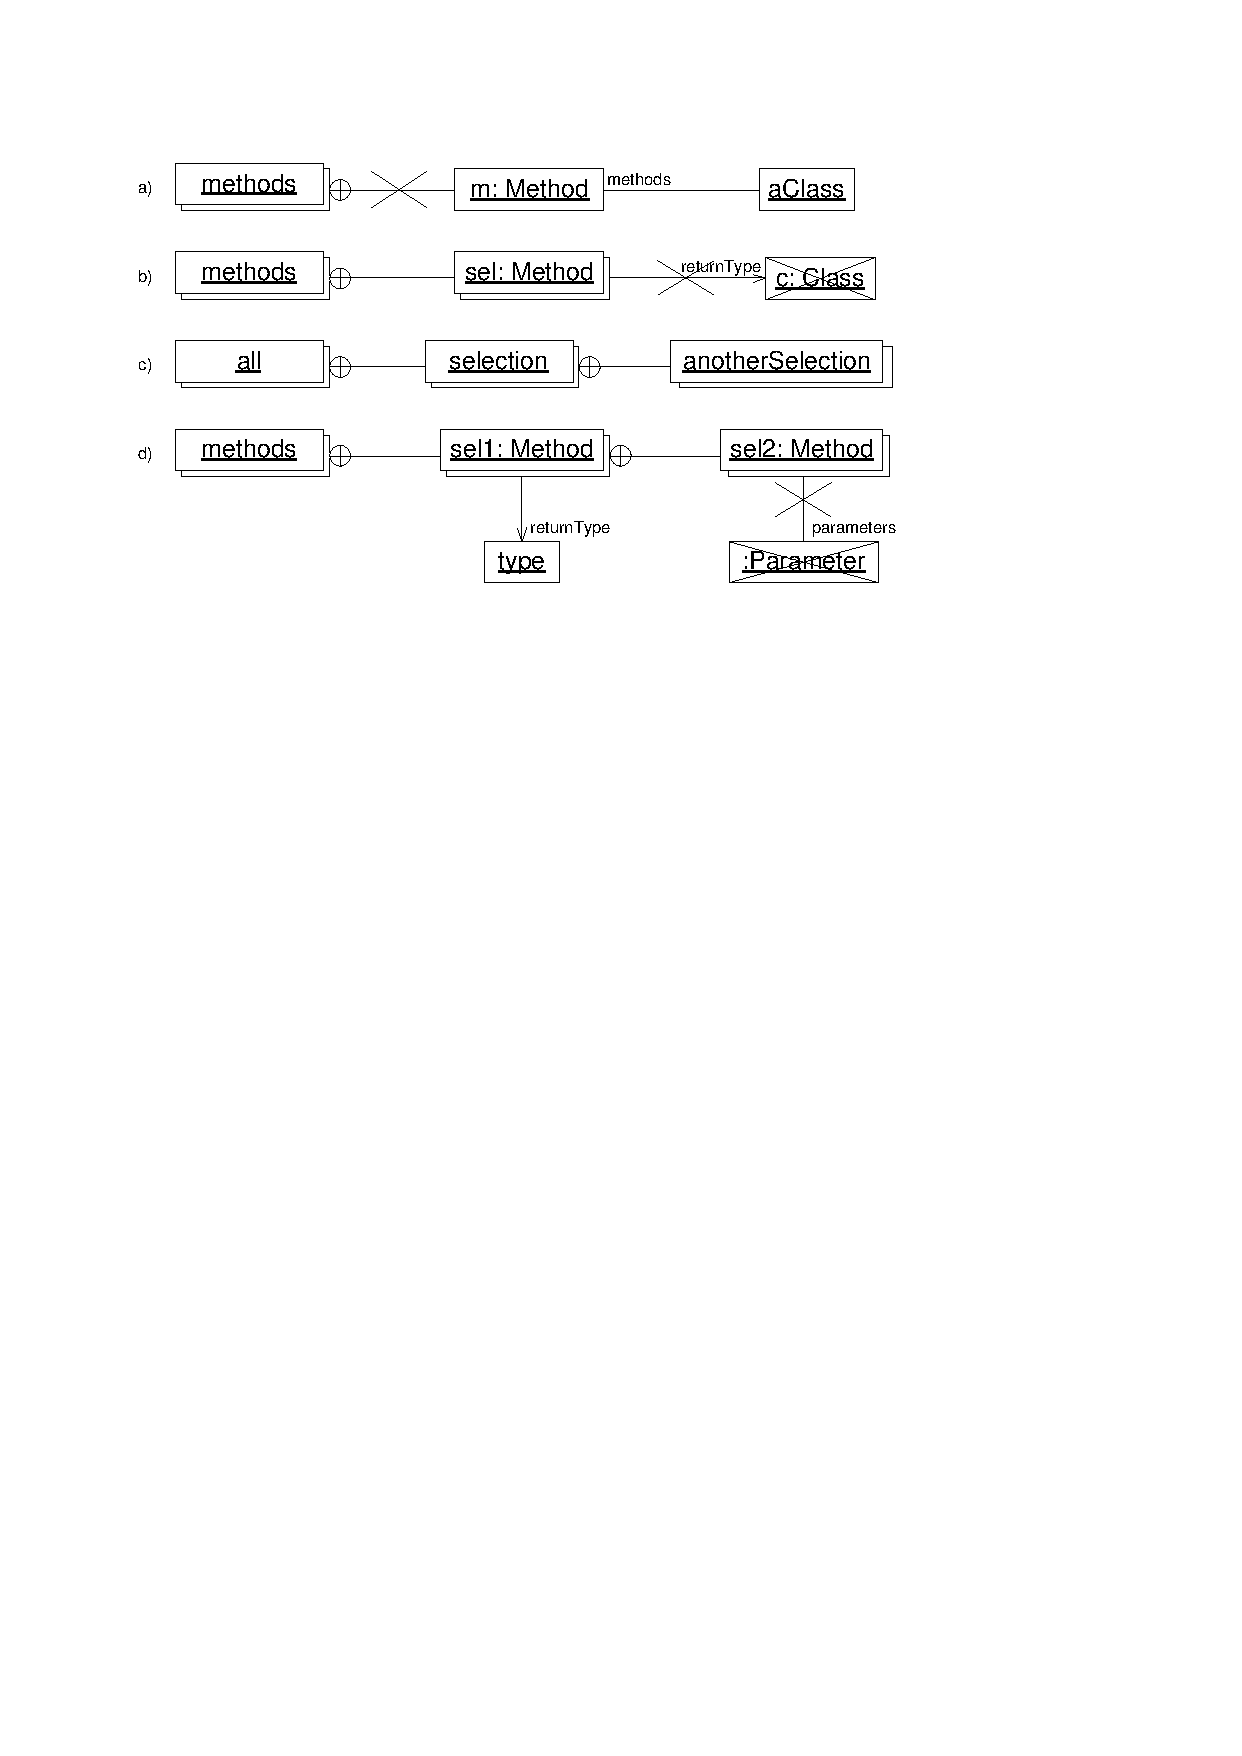
\includegraphics[scale=0.8]{figures/InclusionLinksExamples}
  \caption{Exemplary Uses of Inclusion Links}
  \label{fig:InlucionLinksExamples}
\end{figure}

Inclusion links can be used in combination with link variables.
In Figure~\ref{fig:InlucionLinksExamples} we give some examples for possible uses.
In case a) the story pattern specifies that a \fe{Method} object is to be found which is defined in a class \fe{aClass},
but is not contained in the collection \fe{methods}.
Case b) specifies to find a collection \fe{sel} of \fe{Method} objects which are contained in the collection \fe{methods}
and do not have a return type that is a \fe{Class} object.
The pattern in case c) checks whether a set of objects described by the collection \fe{all} contains another set of objects described by the collection \fe{selection}
which in turn contains another set of objects described by the collection \fe{anotherSelection},
i.e.\ \fe{anotherSelection} is a subset of \fe{selection} and \fe{selection} is a subset of \fe{all}.
The pattern in case d) specifies to find two object sets that are subsets of another set.
First, a collection \fe{sel1} of \fe{Method} objects which have the return type \fe{type} is to be found in the collection \fe{methods}.
Second, a collection \fe{sel2} of \fe{Method} objects which additionaly have no parameters is to be found in the collection \fe{sel1}.


\subsubsection{Feasible Uses of Inclusion Links}
\label{sec:StoryPatterns:inclusion:feasible}

The main difference of inclusion links and link variables is that the source of an inclusion link has to be a collection variable.

Inclusion links can be used with all available binding semantics as described in Section~\ref{sec:StoryPatterns:binding:semantics}.
Consequently, if you replace a negative or optional link in Figures~\ref{fig:negativeObjects} and \ref{fig:optionalObjects}
with a negative or optional inclusion link, you get the feasible combinations of binding semantics used with inclusion links.

Moreover, you get all feasible combinations of binding operators and inclusion links from
Table~\ref{tab:bindingCombinations_links} in Section~\ref{sec:StoryPatterns:binding:operators}.

\begin{figure}[htbp]
  \centering
  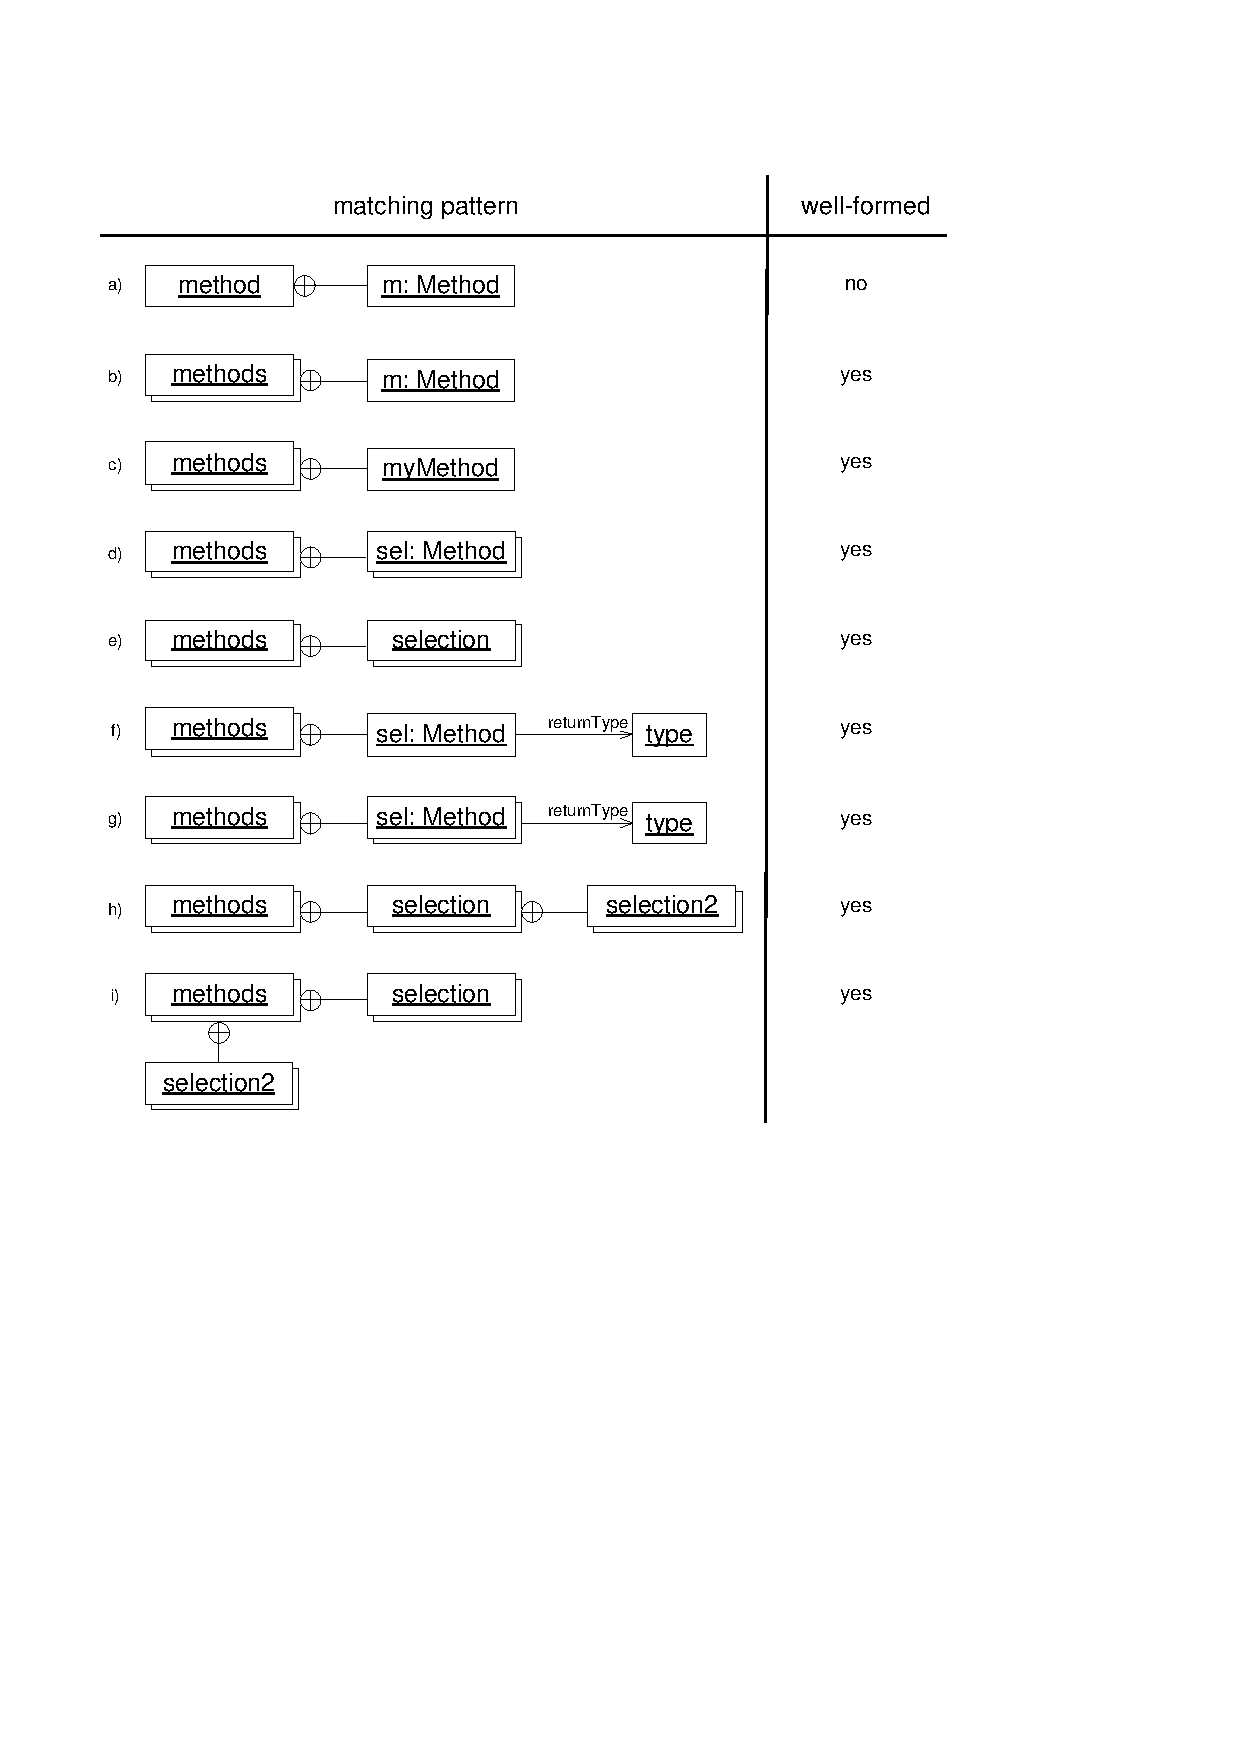
\includegraphics[scale=0.8]{figures/InclusionLinksWellFormedness}
  \caption{Well-formedness of inclusion links}
  \label{fig:InlucionLinkWellFormedness}
\end{figure}

In addition, different combinations of collection variables connected to a bound or unbound variable and
to a single object variable or a collection variable are feasible as illustrated in Figure~\ref{fig:InlucionLinkWellFormedness}.


\subsubsection{Collection Operations with Inclusion Links}
\label{sec:StoryPatterns:inclusion:BagsSetsEtc}

Inclusion links cannot only be used between a collection variable and a single object variable
as shown in Figure~\ref{fig:InlucionLinks} (p.~\pageref{fig:InlucionLinks}),
but also between two collection variables as shown in Figure~\ref{fig:InlucionLinkCollections}.
The semantics for this case are explained in the following.

\begin{figure}[htb]
  \centering
  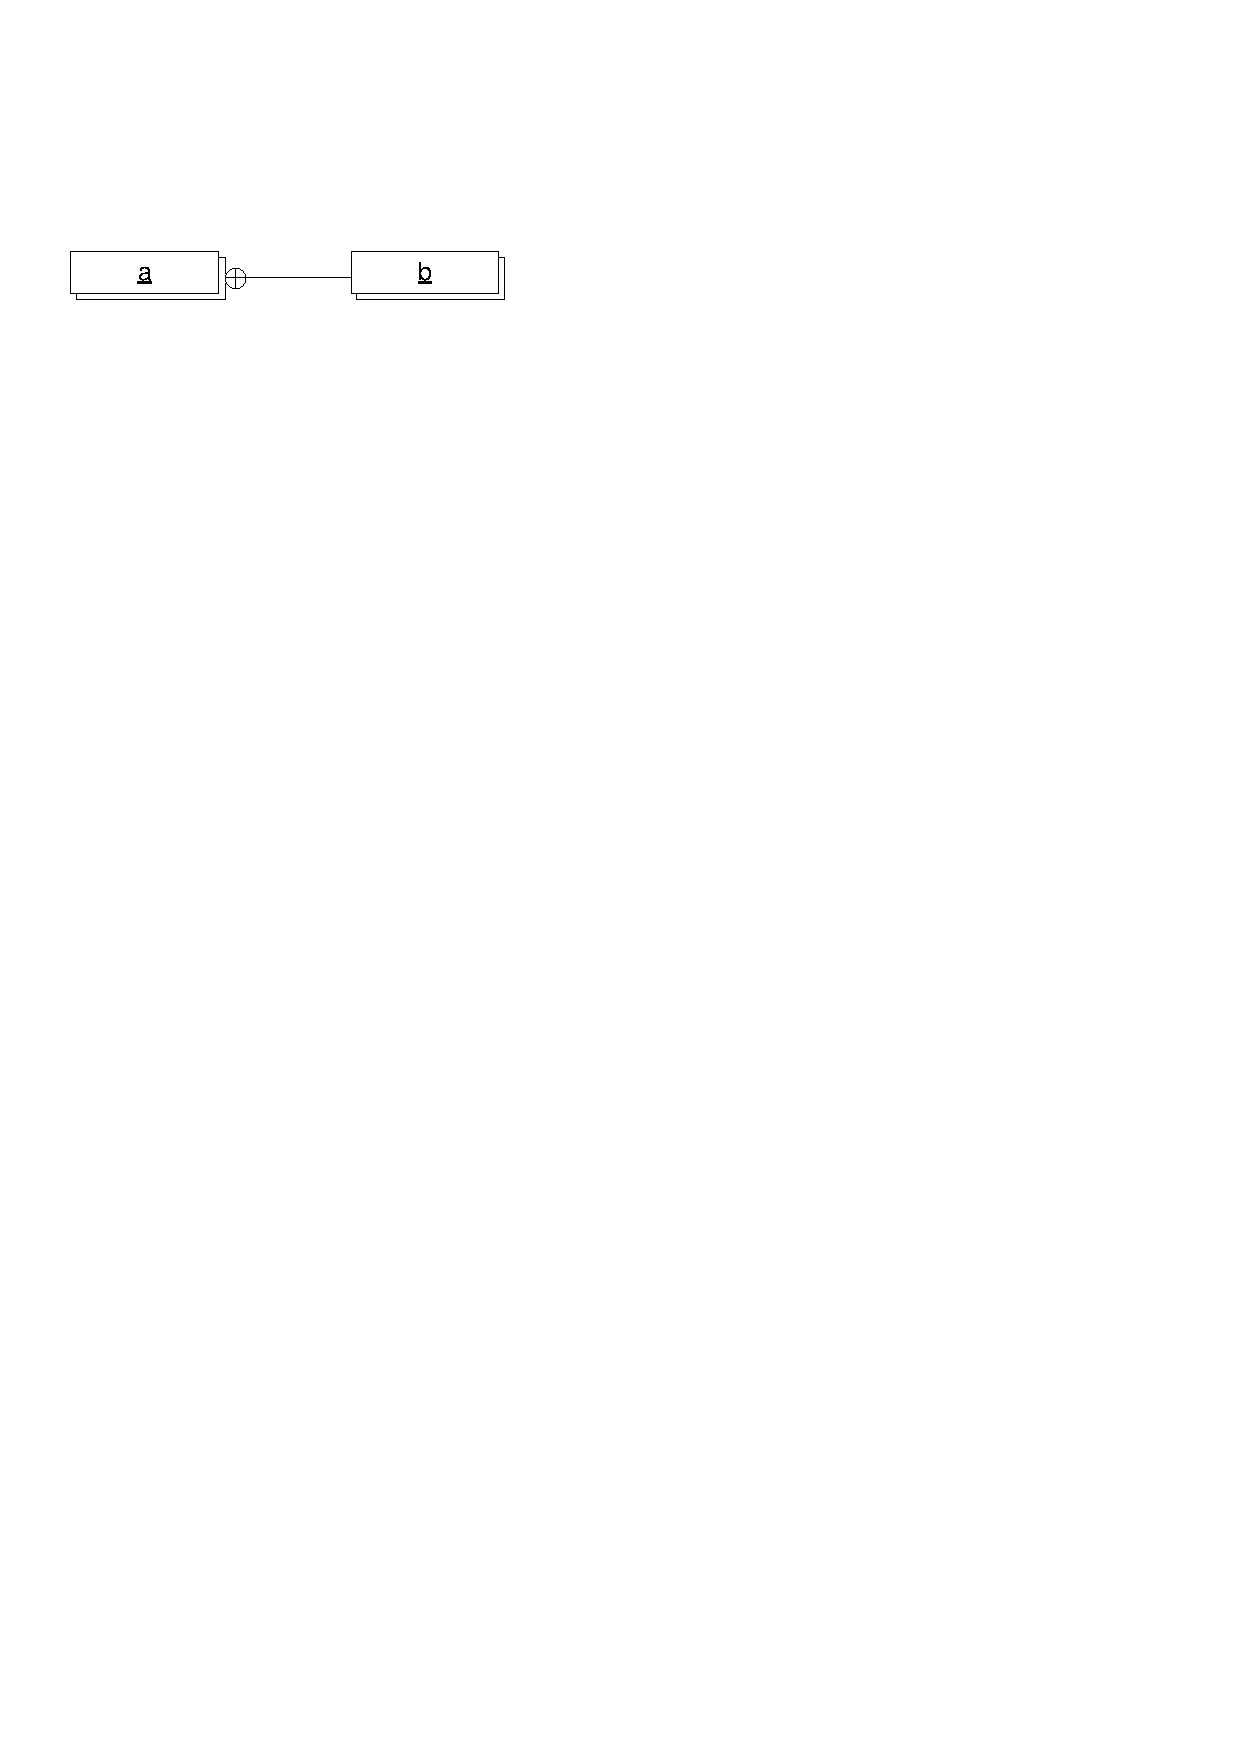
\includegraphics[scale=0.8]{figures/InclusionLinksSetsCheck}
  \caption{Inclusion Link Between Two Collections}
  \label{fig:InlucionLinkCollections}
\end{figure}

An inclusion link between two collection variables represents a containment relation between two sets of objects, i.e.\ between two collections.
In case of the illustration in Figure~\ref{fig:InlucionLinkCollections},
the collection \fe{b} depicts a subset of the set represented by the collection \fe{a} (mathematically $b \subseteq a$).
Interpreting the Figure~\ref{fig:InlucionLinkCollections} as a story pattern,
it describes to check if the elements in collection \fe{b} are also contained in the collection \fe{a}.

In Section~\ref{sec:StoryPatterns:objectsets} we introduced different types of collection variables.
We distinguish between ordered sets and lists.
Sets contain an element mostly once (\emph{unique} property) while lists can contain an element arbitrarily often.
Consequently, the inclusion links between different types of collection variables have different semantics,
which are described in Table~\ref{tab:set_operations_with_inclusion_links}.
The first two columns determine the type of the collections \fe{a} and \fe{b}.
The third column determines if the inclusion link is to be checked, created or removed.
The last column describes the semantics.

The main difference in the semantics of inclusion links stems from the unique or non-unique property of the collections.
If \fe{a} is a set and the binding operator is \fe{CHECK\_ONLY}, we only have to check if all objects in \fe{b} are contained (once) in \fe{a}
(mathematically $a \supseteq b$).
In contrast, if \fe{a} is a list (which can contain the same object arbitrarily often),
we have to ensure that the objects in \fe{b} are not only contained at least once in \fe{a},
but also at least as often as in \fe{b}.
Otherwise, the matching of the story pattern would fail.

An inclusion link with the binding operator \create\ describes to add all objects from \fe{b} to \fe{a}.
If \fe{a} is a set, we only add each object from \fe{b} to \fe{a} if \fe{a} does not already contain it (remember that sets contain each object mostly once).
Since we only have ordered sets, we have to regard the order of the objects in the collections.
We add the objects from \fe{b} to the end of \fe{a} and keep the same order as they had in \fe{b}.
If \fe{a} is a list, we do a similar adding operation, but we add the objects from \fe{b} as often to \fe{a} as they are in \fe{b}.
This can be seen as a concatenation of two lists or the union of two sets (mathematically $a \cup b$).

The binding operator \destroy\ used with an inclusion link and two collections as illustrated in Table~\ref{tab:set_operations_with_inclusion_links}
describes to remove all elements contained in \fe{b} from the collection \fe{a}.
If \fe{a} is a set, we just remove all occurrences of the objects in \fe{b} from \fe{a} and preserve the order of the remaining elements in \fe{a}.
If \fe{a} is a list and \fe{b} is a set, we do quite the same.
Even if an object contained in \fe{b} is contained more than once in \fe{a}, we remove all of its occurrences in \fe{a}.
This comes close to the mathematical relative complement operation (mathematically $a \setminus b$).
If both, \fe{a} and \fe{b} are lists, we only remove as many occurrences of the objects in \fe{b} from \fe{a} as they are available in \fe{b}.
Furthermore, we remove them starting at the beginning of the list \fe{a}.

\begin{table}[htbp]
%  \footnotesize
  \centering
%  \begin{longtable}{|l|l|c|p{4.6cm}|}
  \caption{Inclusion Links Between Two Collection Variables}
  \label{tab:set_operations_with_inclusion_links}
    \begin{tabular}{|l|l|c|p{4.6cm}|}
    \hline
    \textbf{Type of \fe{a}} & \textbf{Type of \fe{b}} & \textbf{Binding Operation} & \textbf{Semantics} \\
    \hline
    \multicolumn{3}{|c}{
      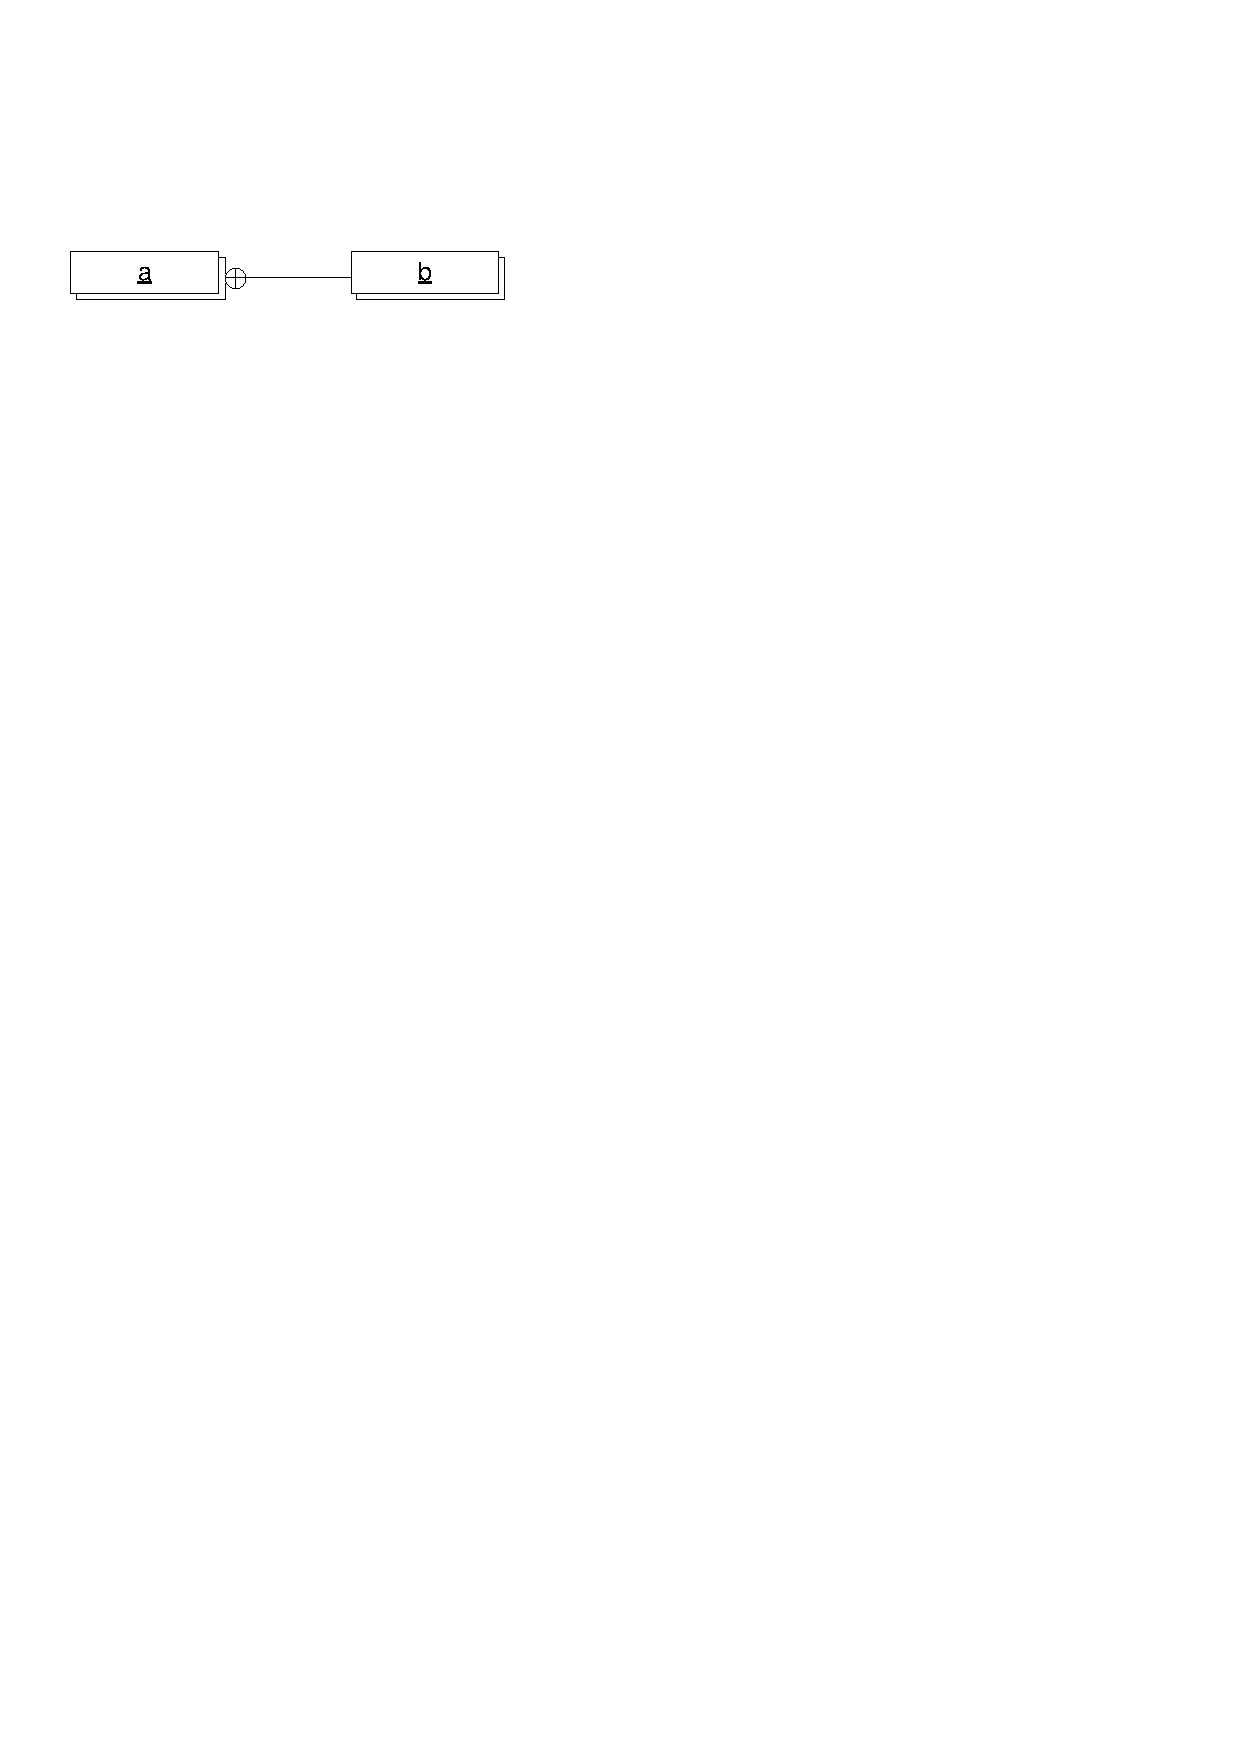
\includegraphics[scale=0.8]{figures/InclusionLinksSetsCheck}
    } & \\
    \hline
    Ordered Set & any & CHECK\_ONLY & Each element in \fe{b} is contained (once) in \fe{a}. \\[0.5em]
    List & any & CHECK\_ONLY & Each element in \fe{b} is contained at least as often in \fe{a} as in \fe{b}.\\
    \hline
    \multicolumn{3}{|c}{
      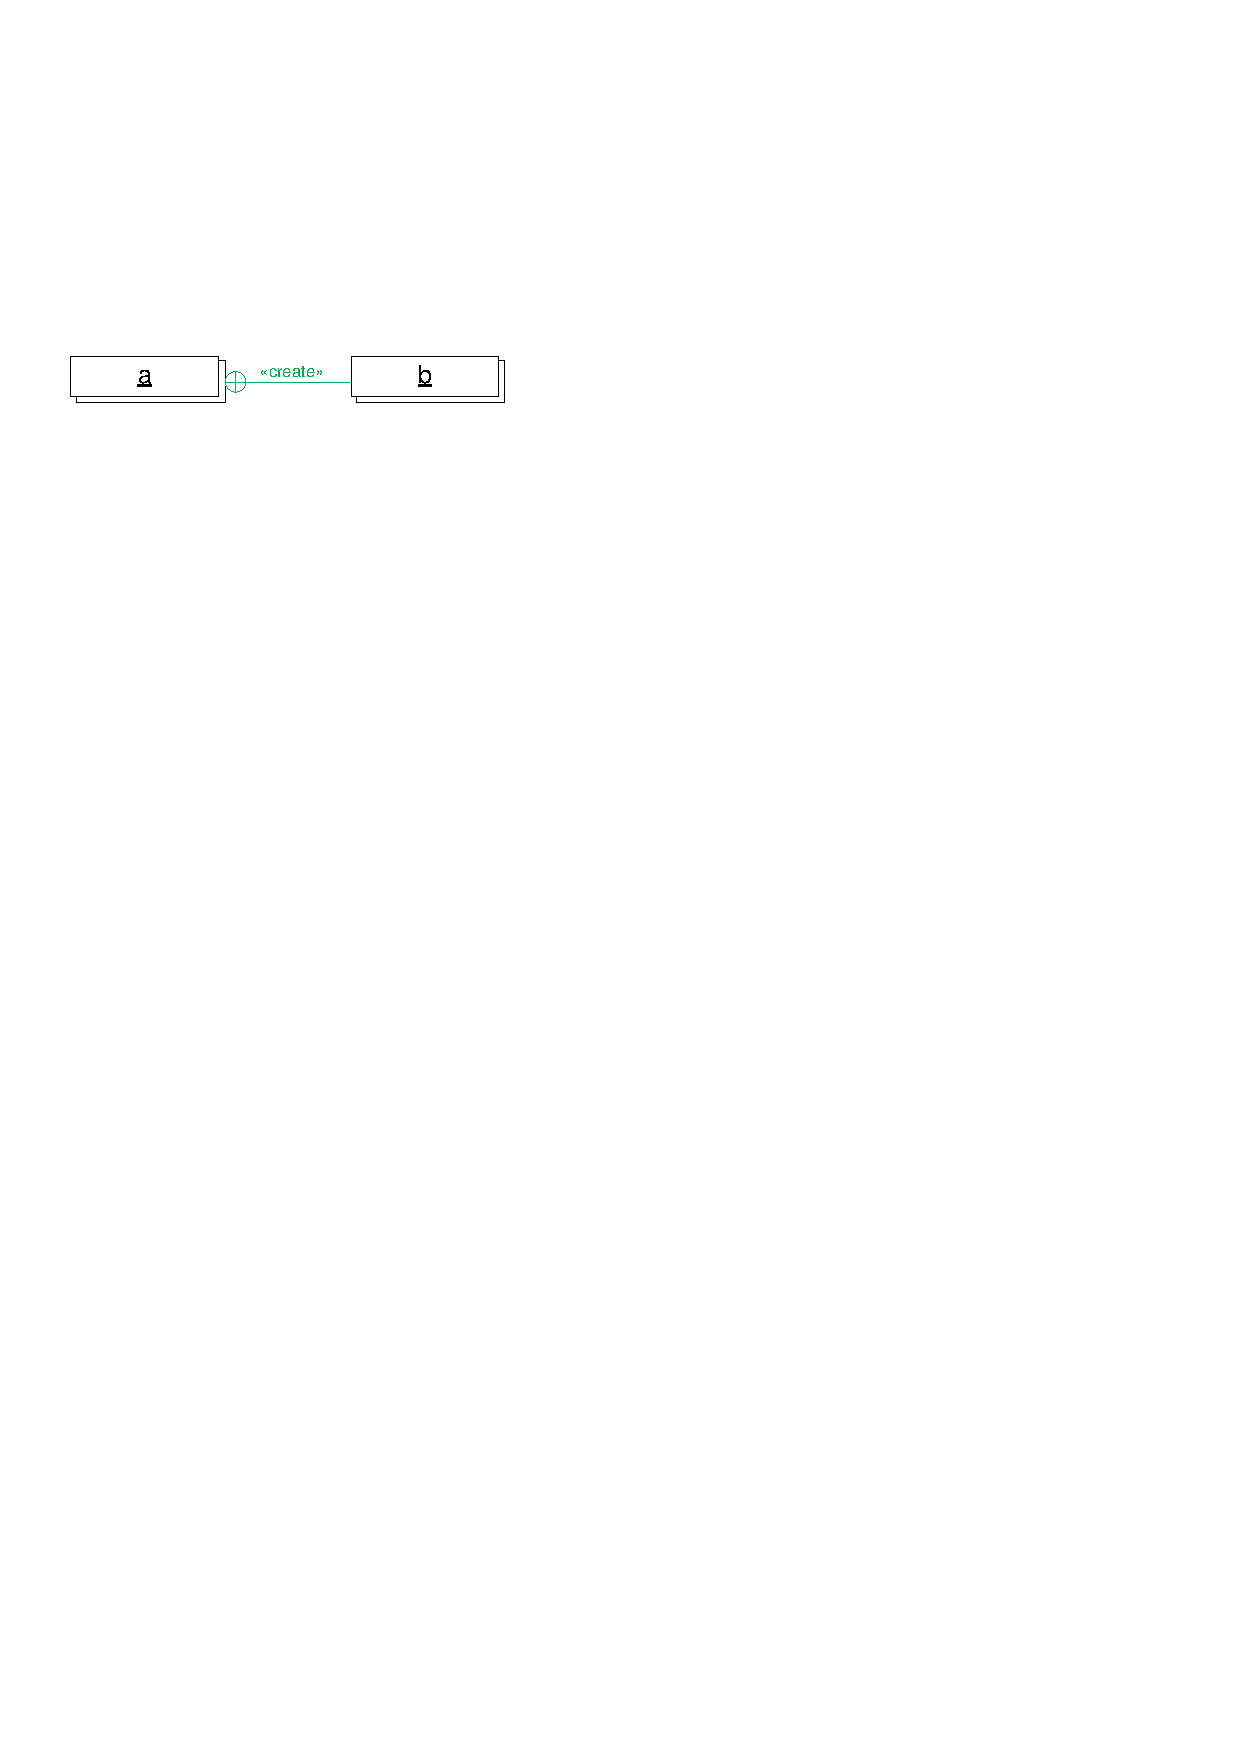
\includegraphics[scale=0.8]{figures/InclusionLinksSetsCreate}
    } & \\
    \hline
    Ordered Set & any & CREATE & Add all elements from \fe{b} to \fe{a} that are missing in \fe{a} to the end of \fe{a}, preserving the order of elements in \fe{b}.\\[0.5em]
    List & any & CREATE & Add all elements from \fe{b} to \fe{a} to the end of \fe{a}, preserving the order of elements in \fe{b}.\\
    \hline
    \multicolumn{3}{|c}{
      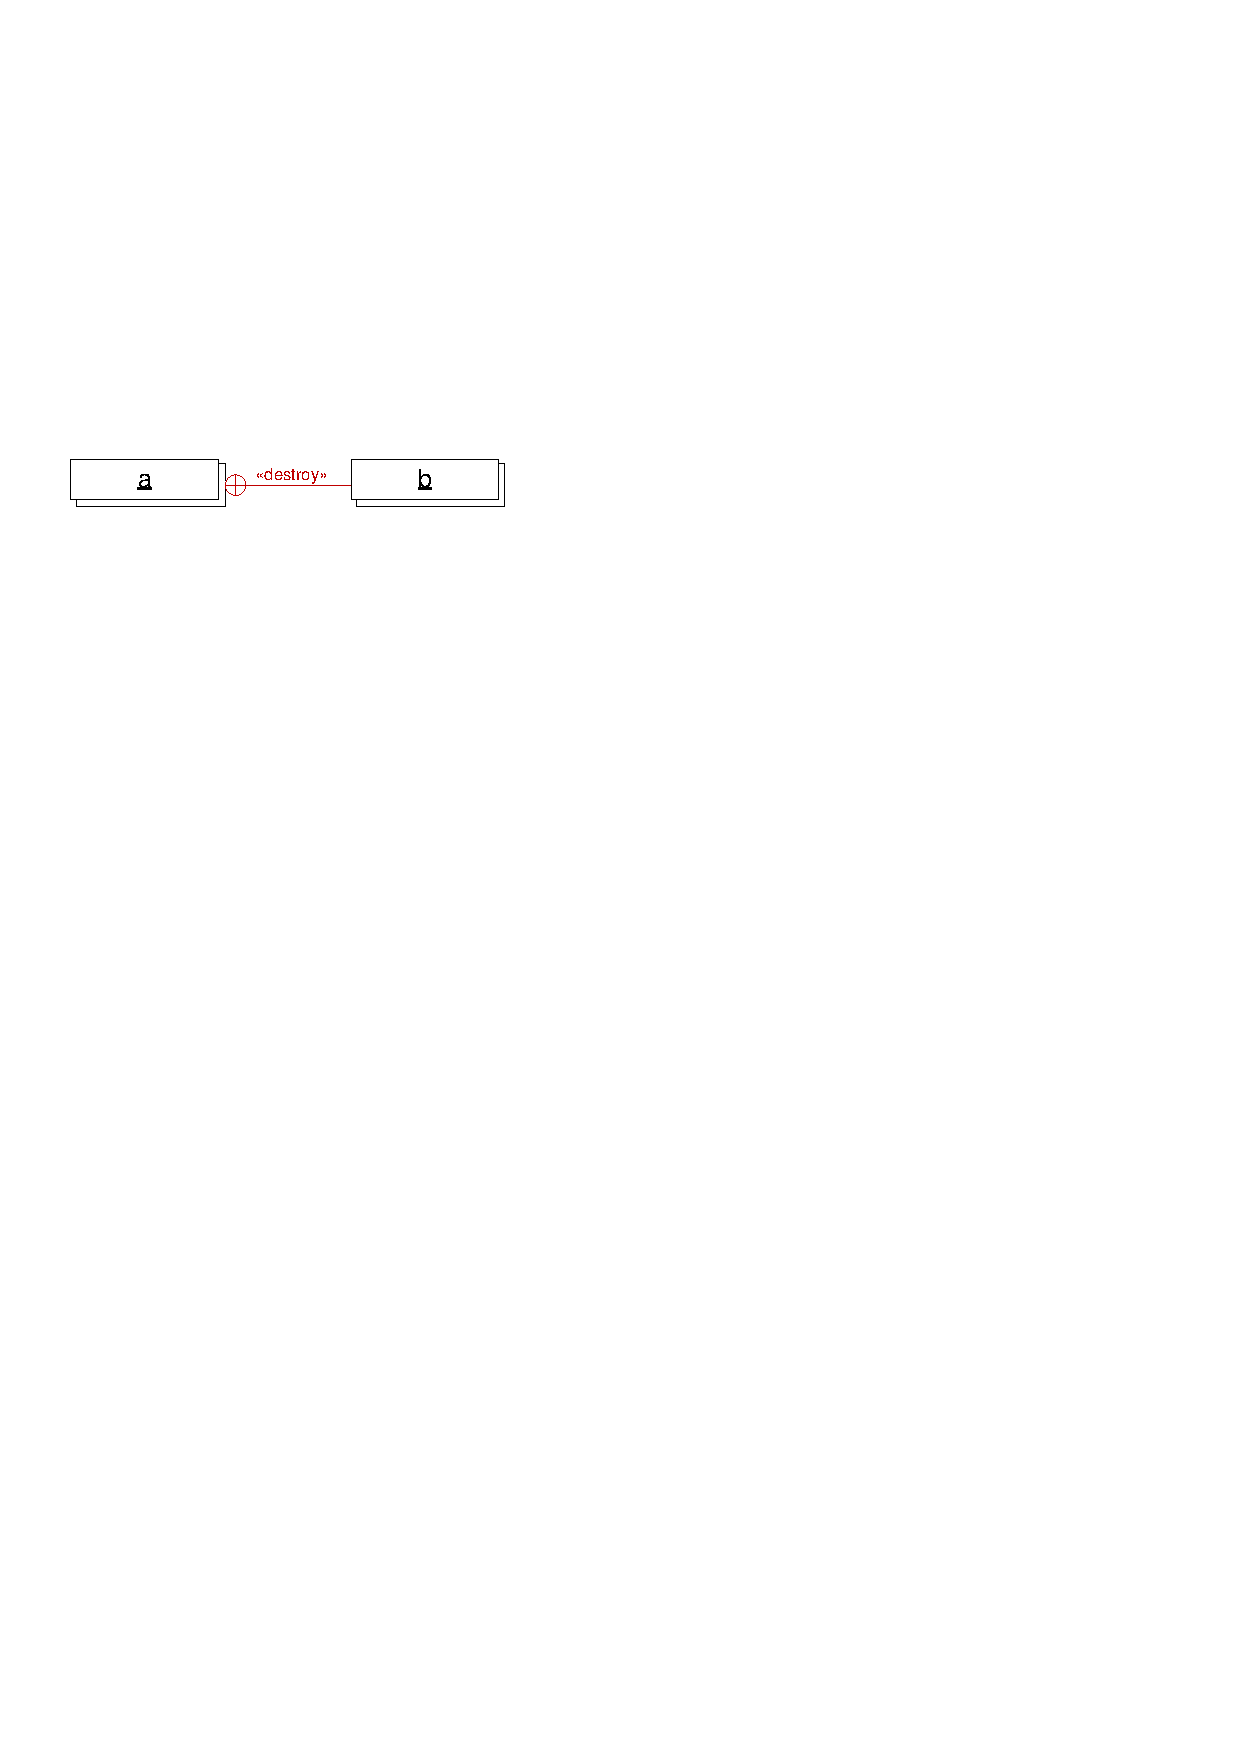
\includegraphics[scale=0.8]{figures/InclusionLinksSetsDestroy}
    } & \\
    \hline
    Ordered Set & any & DESTROY & Remove all elements in \fe{b} from \fe{a}, preserve the order of remaining elements in \fe{a}.\\[0.5em]
    List & Ordered Set & DESTROY & Remove \emph{all} occurrences of elements contained in \fe{b} from \fe{a}, preserve the order of remaining elements in \fe{a}.\\[0.5em]
    List & List & DESTROY & Starting at the beginning of the list \fe{a}, for each element in \fe{b} remove as many occurrences of the element in \fe{a} as it is available in \fe{b}, preserve the order of remaining elements in \fe{a}.\\
    \hline
    \end{tabular}
%  \end{longtable}
\end{table}

\begin{figure}[htb]
  \centering
  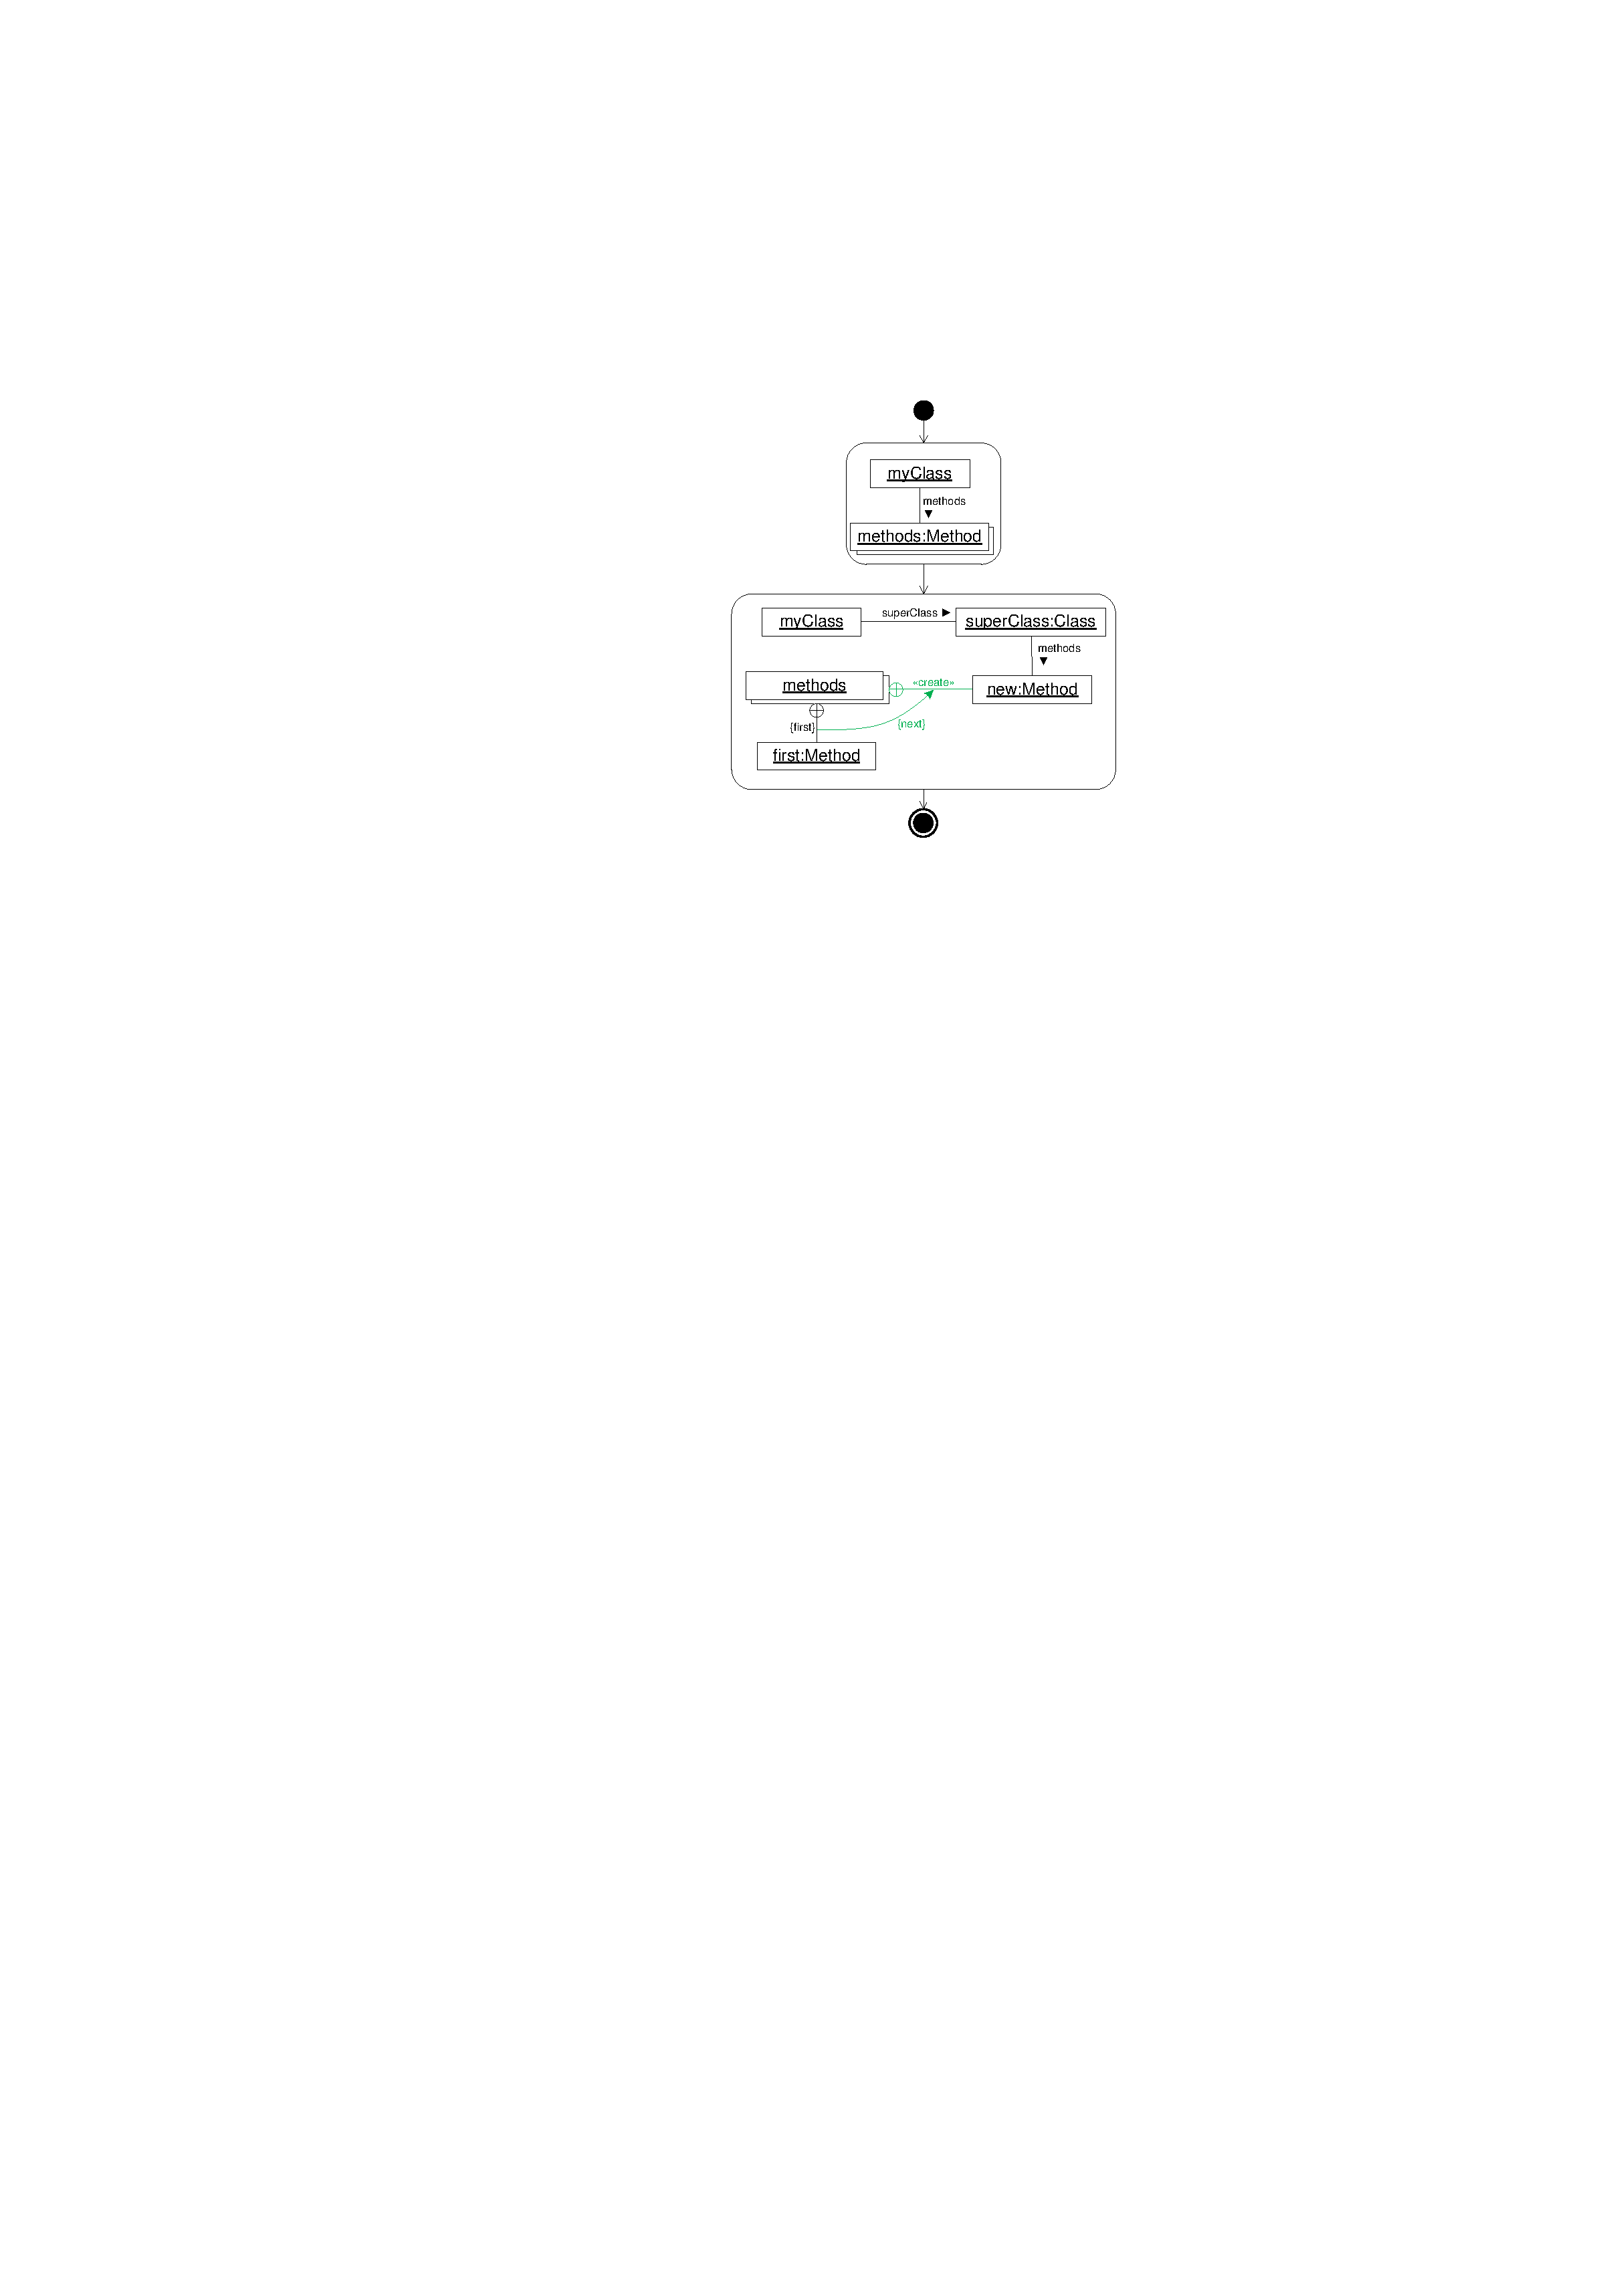
\includegraphics[scale=.8]{figures/LinkConstraints1}
  \caption{Inclusion Links With Link Order Constraints}
  \label{fig:collectionsLinkConstraints}
\end{figure}

Similar to the link constraints described in Section~\ref{sec:StoryPatterns:linkConstraints}, these can also be used with inclusion links.
An exemplary use is illustrated in the story diagram in Figure~\ref{fig:collectionsLinkConstraints}.
We will explain story diagrams in more detail in Section~\ref{sec:StoryDiagrams}.
Here, the story diagram describes the sequential execution of two story patterns.

In the first story pattern (the upper one), a set of \fe{Method} objects is collected from a given class \fe{myClass} and stored in the collection \fe{methods}.
In the next story pattern, a superclass of \fe{myClass}, a method in this superclass and the first method in the collection \fe{methods} are matched.
In case of a successful matching the newly matched method \fe{new} is added to the collection \fe{methods}.
The link constraint \fe{\text\{next\text\}} determines to add this method to the ordered collection in such a way
that the method \fe{new} directly follows the method \fe{first} in the collection \fe{methods}.



%\ext %--- Comment this line to include paths into the document
{ 
\subsection{Paths [MCP]}
\label{sec:StoryPatterns:paths}
} %--- End of paths subsection


%\ext  %--- Comment this line to include pattern fragments into the document
{
\subsection{Pattern Fragments [MCP]}

patterns contained in other patterns, negative, semantics? review enhanced story patterns from Diss Florian Klein

\todomcp{Should contained pattern be marked as forEach? Idea for semantics: first the part of the pattern outside the forEach pattern is matched, then the forEach subpattern is applied to any match that may be located, the variables bound in a forEach subpattern may not be used in subsequent activities}

\todoch{The transformations diagrams that Matthias Meyer developed in his Diss contain so-called iterated parts that are essentially the same as a for-each fragment. We should check his semantics.}

\tododt{This is somewhat confusing.
As I understand them, subpatterns are ordinary story patterns within another story pattern.
They are surrounded by a fragment box and can be labeled with a name (see Figure~\ref{fig:labeledSubPattern}).
Special types of such subpatterns are negative application condition fragments (NACs), set fragments, and optional fragments.
As far as I know, we did not plan to add $\forall$ and $\exists$ fragments, did we?
These are only used in SDDs and TSSDs which are constraint languages.
}

\begin{figure}[htbp]
  \centering
  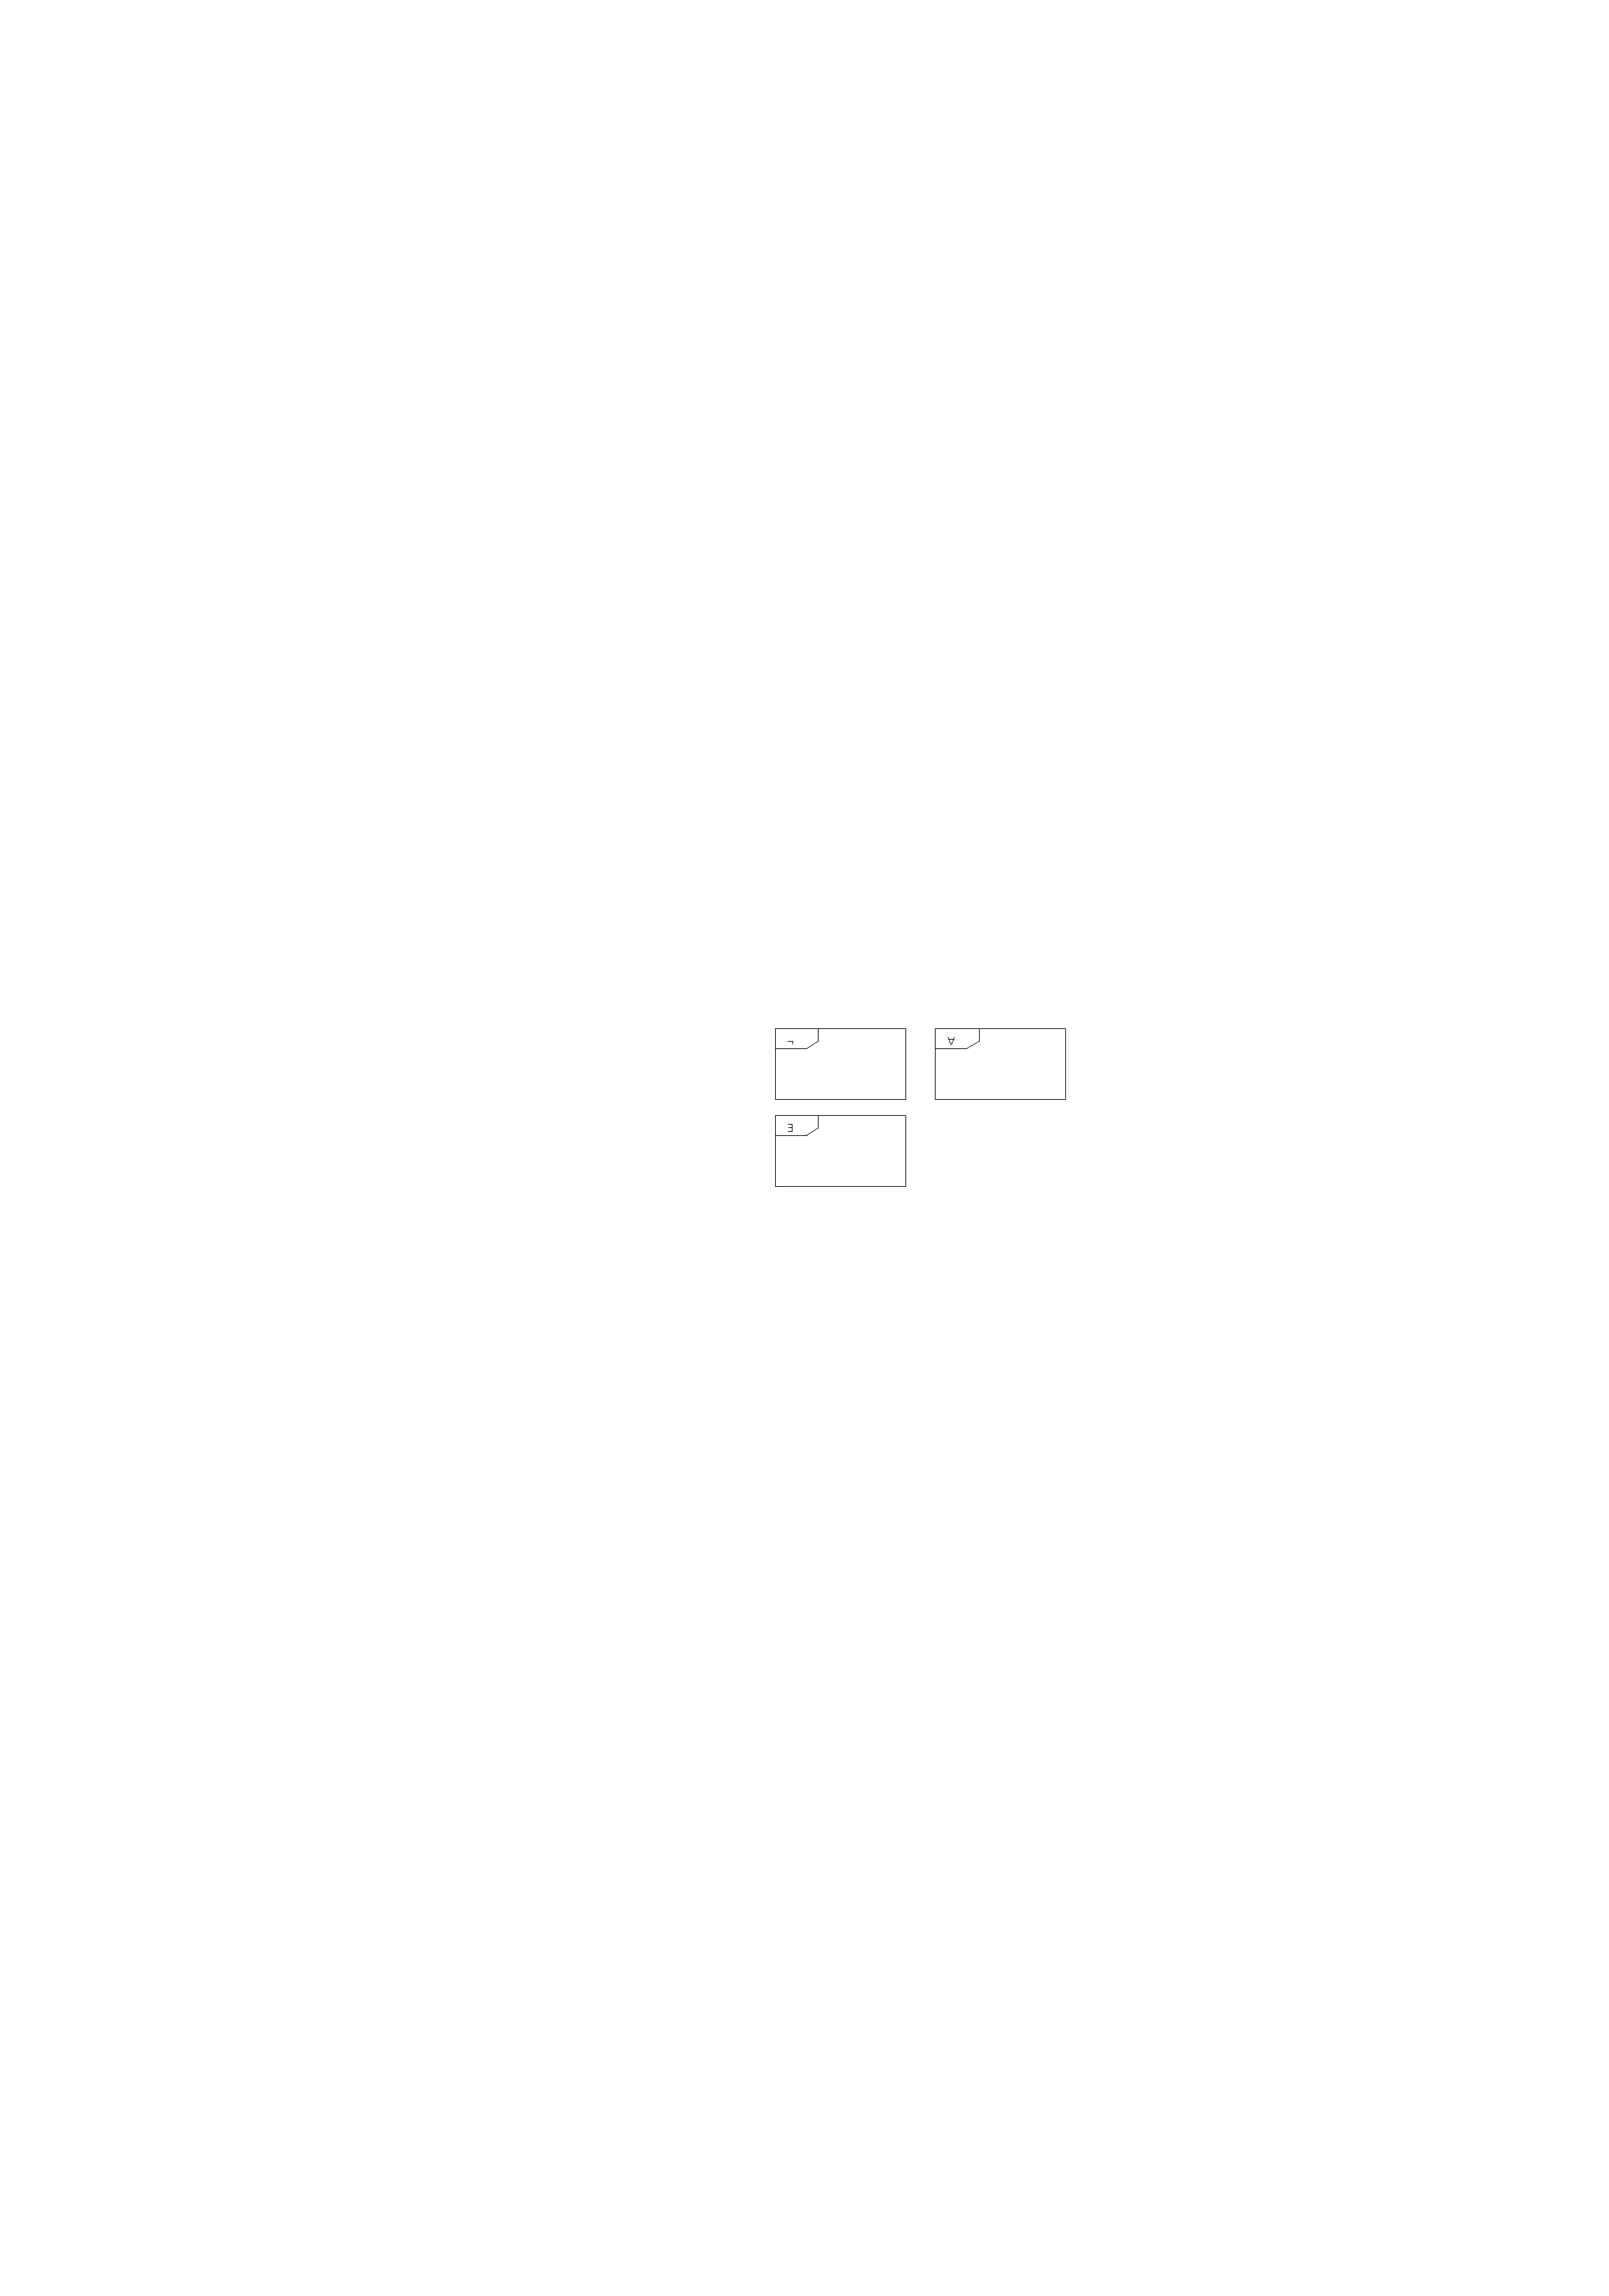
\includegraphics[scale=1.0]{figures/ContainedPattern}
  \caption{Different Kinds of Contained Patterns}
  \label{fig:containedPattern}
\end{figure}

\todomcp{Should contained pattern be marked as optional? Is currently possible in the metamodel. Idea for semantics: Whole pattern must be found, if found, variables may be used in subsequent activities, if pattern may not be found as a whole, matching still succeeds but all variables in the subpattern are not bound in subsequent activities.}
\tododt{I would say, contained patterns are mandatory in general (or are NAC/optional/set in case of the according fragment).}

\begin{figure}[htbp]
  \centering
  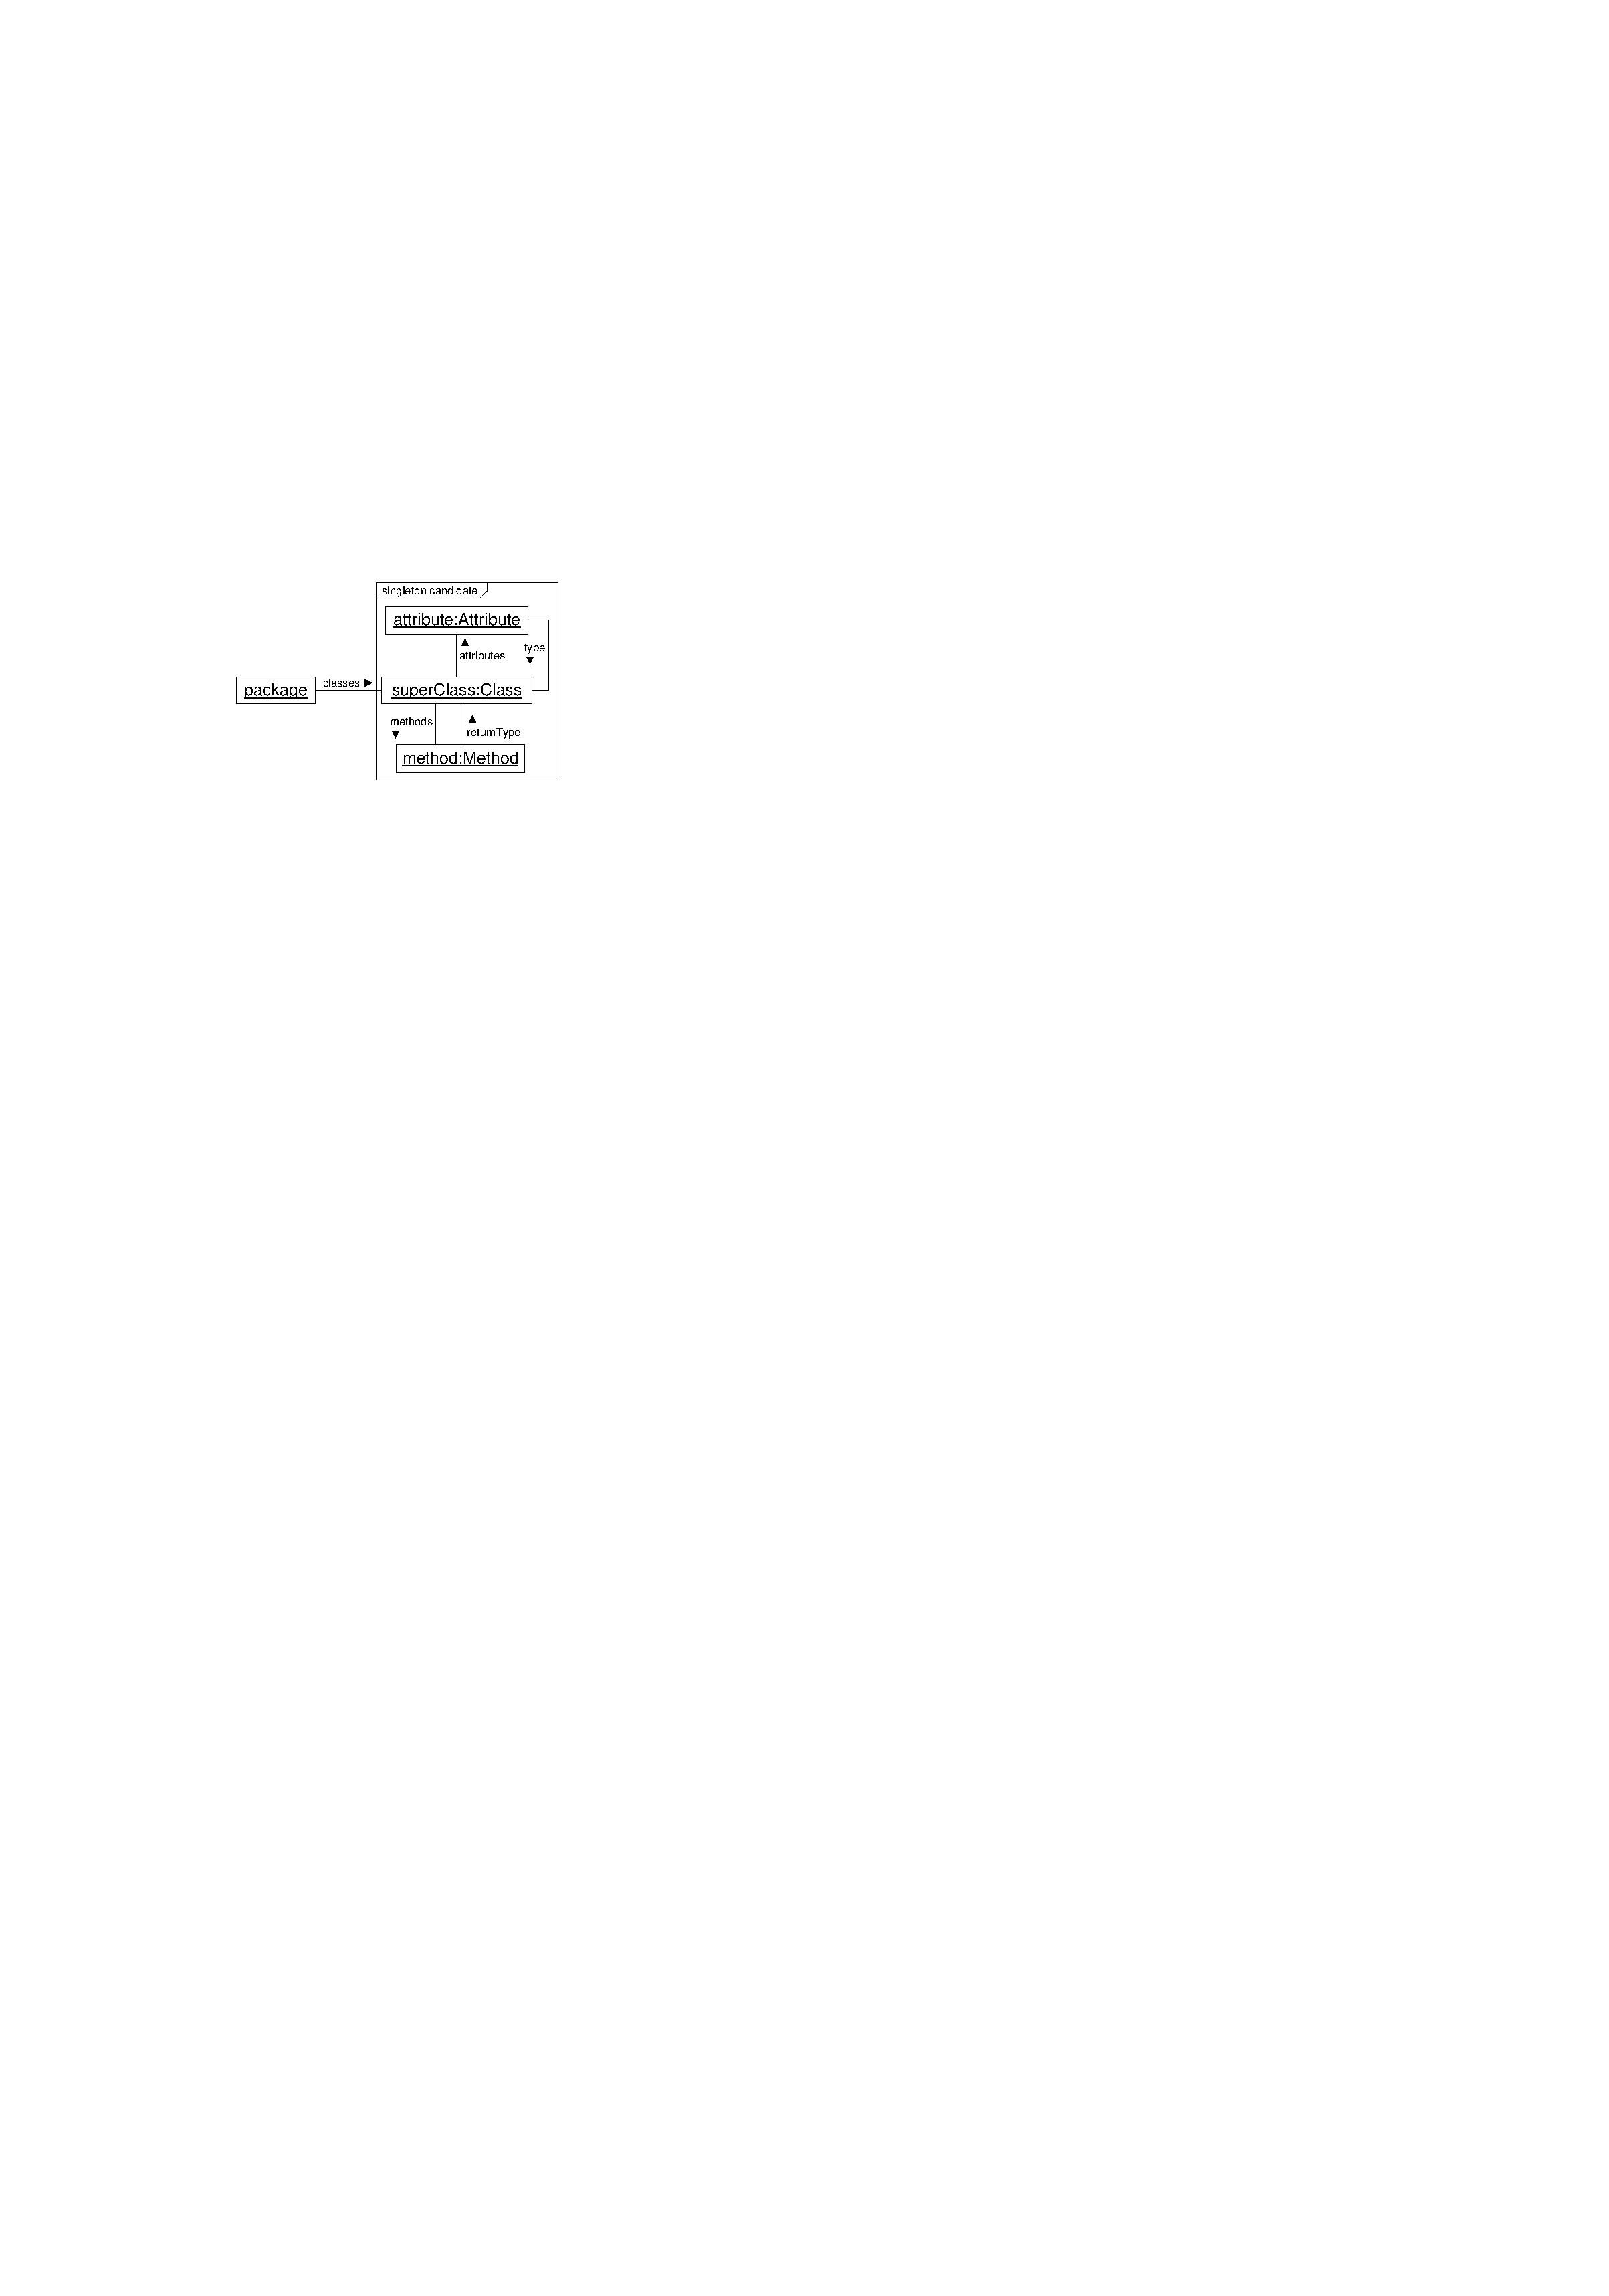
\includegraphics[scale=1.0]{figures/SubPatterns2}
  \caption{Labeled sub pattern}
  \label{fig:labeledSubPattern}
\end{figure}

\begin{figure}[htbp]
  \centering
  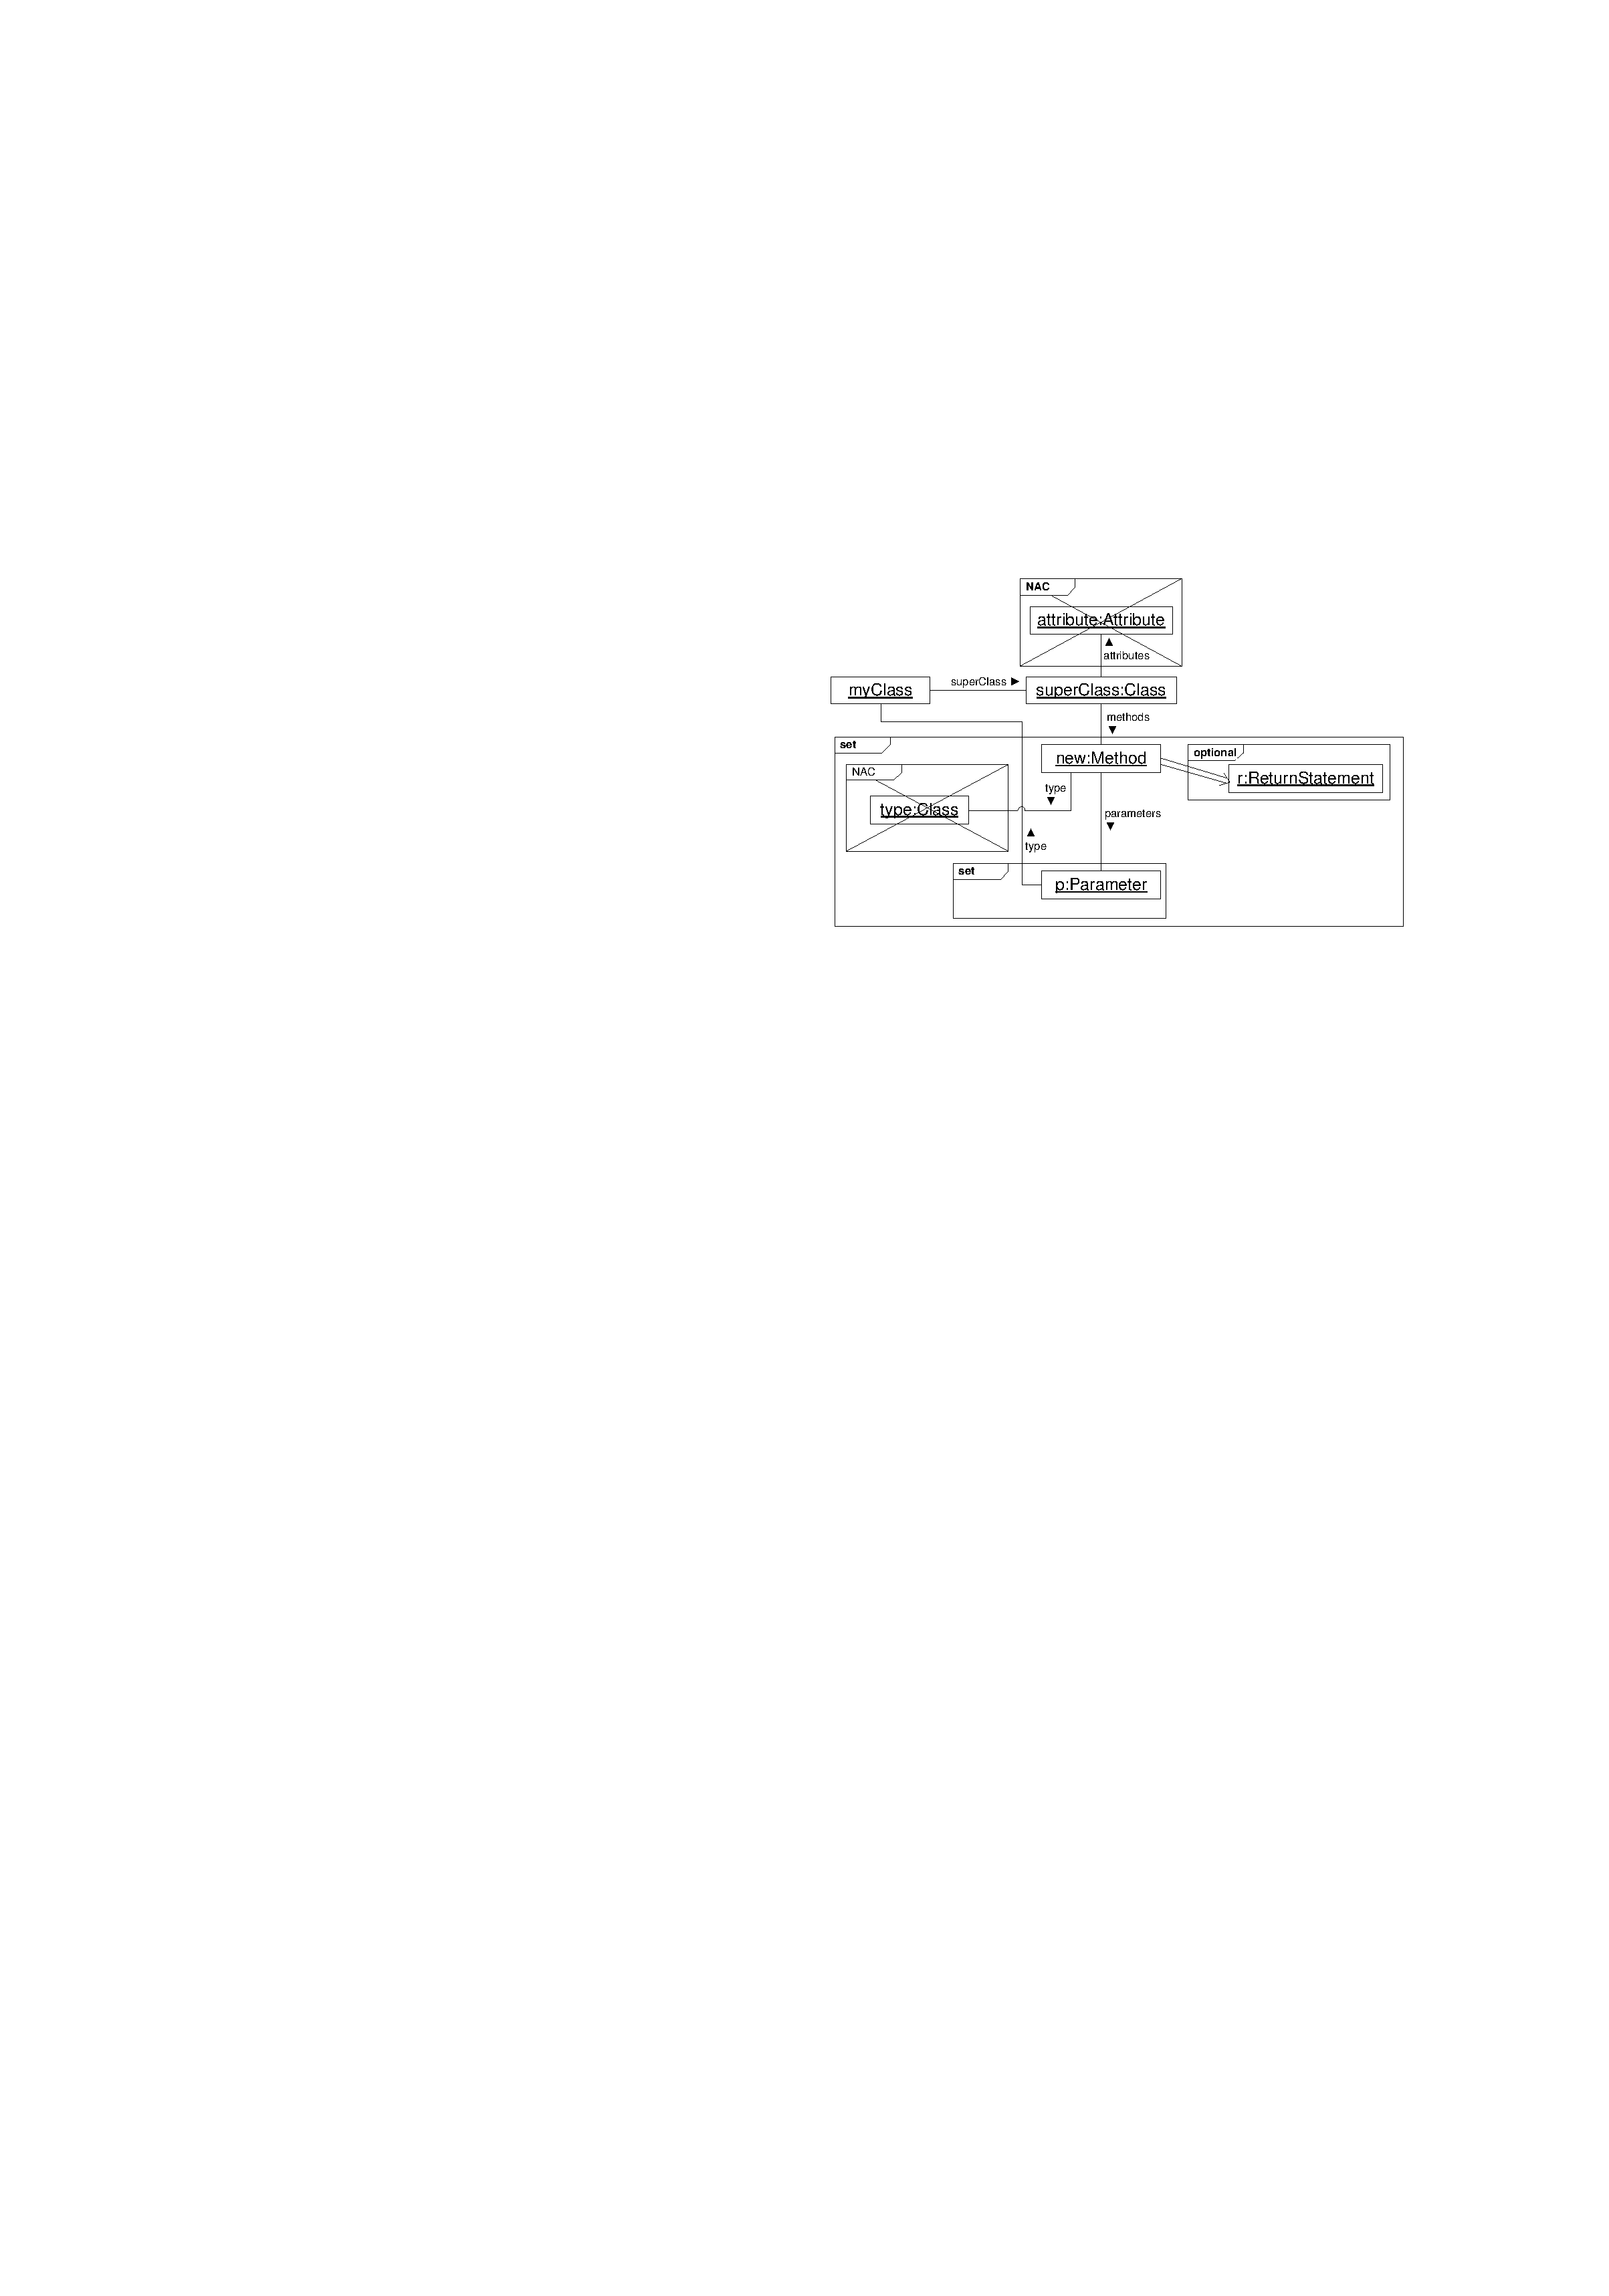
\includegraphics[scale=1.0]{figures/SubPatterns1}
  \caption{Hierarchies of NAC, set, and optional sub patterns}
  \label{fig:subPatternHierarchies}
\end{figure}

\todomcp{How deep may patterns be nested? What is the semantics of alternating binding semantics of sub-patterns, e.g. negative in optional in negative and so on.}
\tododt{I would prefer to allow arbitrarily deep nestings and would suggest to interpret the fragments in the order from outside to inside. Example (see Figure~\ref{fig:subPatternHierarchies}): You match a super class \emph{superClass} of \emph{myClass} and ensure that \emph{superClass} has no attribute. Then you you match all methods \emph{new} (outer set fragment) that have no class as their type (enclosed NAC fragment). Now you match for each of these methods all parameters (enclosed set fragment) that have \emph{myClass} as their type. Furthermore, you try to find a path from the matched \emph{new} method to a return statement (optional fragment).}

} %--- End of pattern fragment section


